\documentclass[11pt,letterpaper]{article}
\usepackage{geometry}
\geometry{margin=0.5in}
\usepackage{graphicx}
\usepackage{placeins}
\usepackage{amsmath}
\usepackage{multirow}
\usepackage{multicol}
\usepackage{booktabs}
\usepackage{float}
\usepackage{subcaption}


\setlength{\parindent}{0pt}
\setlength{\parskip}{0.5em}

%make lists tighter
\usepackage{enumitem}
\setlist{nolistsep}

%reduce spacing before and after section
\usepackage{titlesec}
\titlespacing*{\section}{0pt}{0\baselineskip}{0\baselineskip}
\titlespacing*{\subsection}{0pt}{0\baselineskip}{0\baselineskip}
\titlespacing*{\subsubsection}{0pt}{0\baselineskip}{0\baselineskip}

%reduce list spacing
\setlist{nosep}

\usepackage[hidelinks]{hyperref}

\title{Lab 2 - Cloud Data, Stat 214, Spring 2026\vspace{-2em}}

% submission must not contain any of your names
% but feel free to make a version for yourself with your names on it
% \author{Anonymous}

\begin{document}
\maketitle

\section{Introduction}
\label{sec:intro}

Accurate cloud detection is a critical prerequisite for climate modeling and remote sensing analysis, but it also presents challenges when performed over Arctic regions due to the similar remote sensing characteristics of clouds and ice/snow-covered surfaces \cite{Shi}. To tackle this challenge, work has been done by Shi et al. to utilize NASA's Multiangle Imaging SpectroRadiometer (MISR) imagery. This technology captures radiation measurements from different camera angles which exploits the fact that the radiation measurements tend to scatter for cloudy regions. Furthermore, Shi et al. developed three features from these measurements to aid in the detection of clouds: CORR (the correlation of radiation measurements at different angles), SD (the standard deviation within groups of MISR's AN camera), and NDAI (normalized difference angular index).

For this project, we are provided with a set of 164 images taken over the Arctic using the MISR technology. Within each pixel of each image, radiation measurements from five cameras (AN, AF, BF, CF, DF) corresponding to five different angles $(0^{\circ}, 26.1^{\circ}, 45.6^{\circ}, 60.0^{\circ}, 70.5^{\circ})$ are stored. The three features engineered by Shi et al. are also captured for each pixel. Of these 164 images, only three have expert-drawn labels for cloudy and non-cloud regions.

Our goal for this project is to develop a robust algorithm for cloud detection. To accomplish this, we first conduct an exploratory data analysis to understand variable distributions, spatial structure, and inter-feature relationships (Section \ref{sec:EDA}). Next, we engineer an expanded feature set from the original features and train an autoencoder on the unlabeled images to extract additional features that will help in maximizing predictive power (Section \ref{sec:feat_eng}). We then train and evaluate four different classification models: Logistic Regression, Random Forest, Gradient Boosted Trees, and $k$-Nearest Neighbors (Section \ref{sec:model}). Finally, we evaluate our best model and conduct stability and post-hoc analyses.

\section{EDA}
\label{sec:EDA}

\subsection{Dataset Overview}

For our EDA, we will be analyzing the three images with expert labels to understand the relationship between the features provided and cloud presence. For these images, each pixel is labeled as having either a cloud (+1), no cloud (-1), or unlabeled (0). Figure \ref{fig:expert_labels} shows the expert labels for the presence of clouds.

\begin{figure}[!htbp]
    \centering
    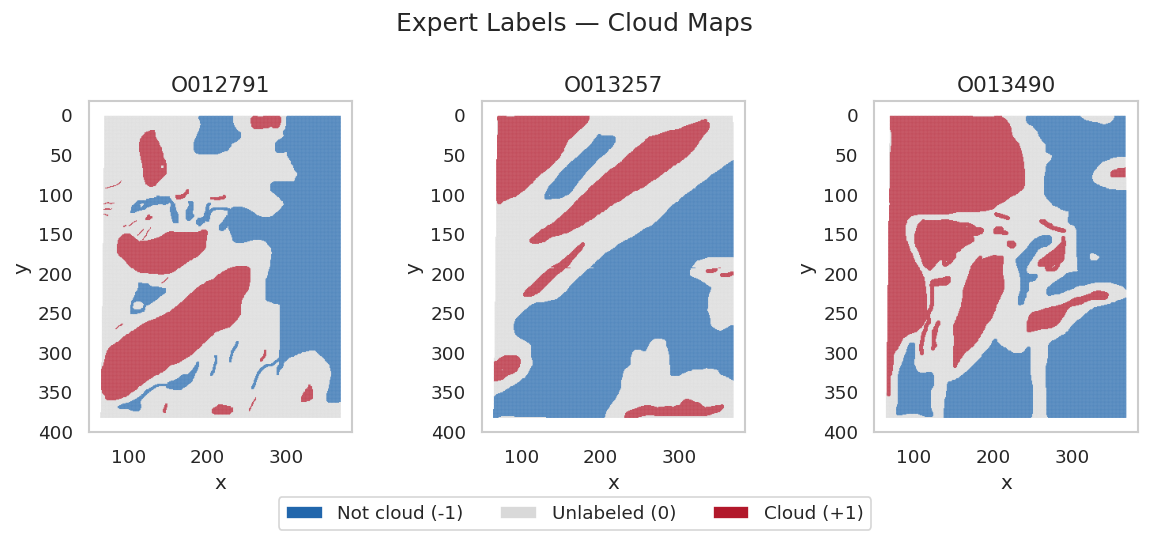
\includegraphics[width=0.75\textwidth]{./figures/image_label_plots.png}
    \caption{Expert Labels of Images}
    \label{fig:expert_labels}
\end{figure}
\FloatBarrier

From the images, we see that there is a large spatial dependency for determining cloudiness. The cloudy/non-cloud regions form clusters, so if we can identify a region's border as cloudy/not cloudy, it's very likely that we can identify the interior points as well. However, both Table \ref{table:cloud_coverage} and even the expert-labeled images present some challenges. First, we see that many of the regions are still unlabeled, further limiting our ability to differentiate between clouds/non-clouds. Second, we note that the percentage of clouds varies by image. This imbalance may result in a model's ``base" predicted probability of a cloud being shifted depending on which images are used for training/testing. This implication will be further discussed in Section \ref{sec:model}.

\begin{table}[h!]
\centering
\begin{tabular}{ccccc}
\toprule
\textbf{Image Name} & \textbf{\% Cloudy} & \textbf{\% Not Cloudy} & \textbf{\% Unlabeled} & \textbf{Pixel Count} \\ 
\midrule
O012791 & 18.5 & 29.2 & 52.4 & 114,973 \\
O013257 & 17.8 & 43.8 & 38.4 & 115,000 \\
O013490 & 34.1 & 37.2 & 28.6 & 115,032 \\
\bottomrule
\end{tabular}
\caption{Cloud Coverage per Image}
\label{table:cloud_coverage}
\end{table}
\FloatBarrier

\subsection{Data Exploration}

For the purposes of this data exploration, we removed the unlabeled pixels. The reason for doing so is that for now, we are only interested in how the variables differ by cloud label. We eventually add the unlabeled images back in when we conduct our feature engineering, and then remove them again during the model-building phase, but for now, we began our exploration by observing distributions of each variable, separated by cloud class.

\begin{figure}[!htbp]
    \centering
    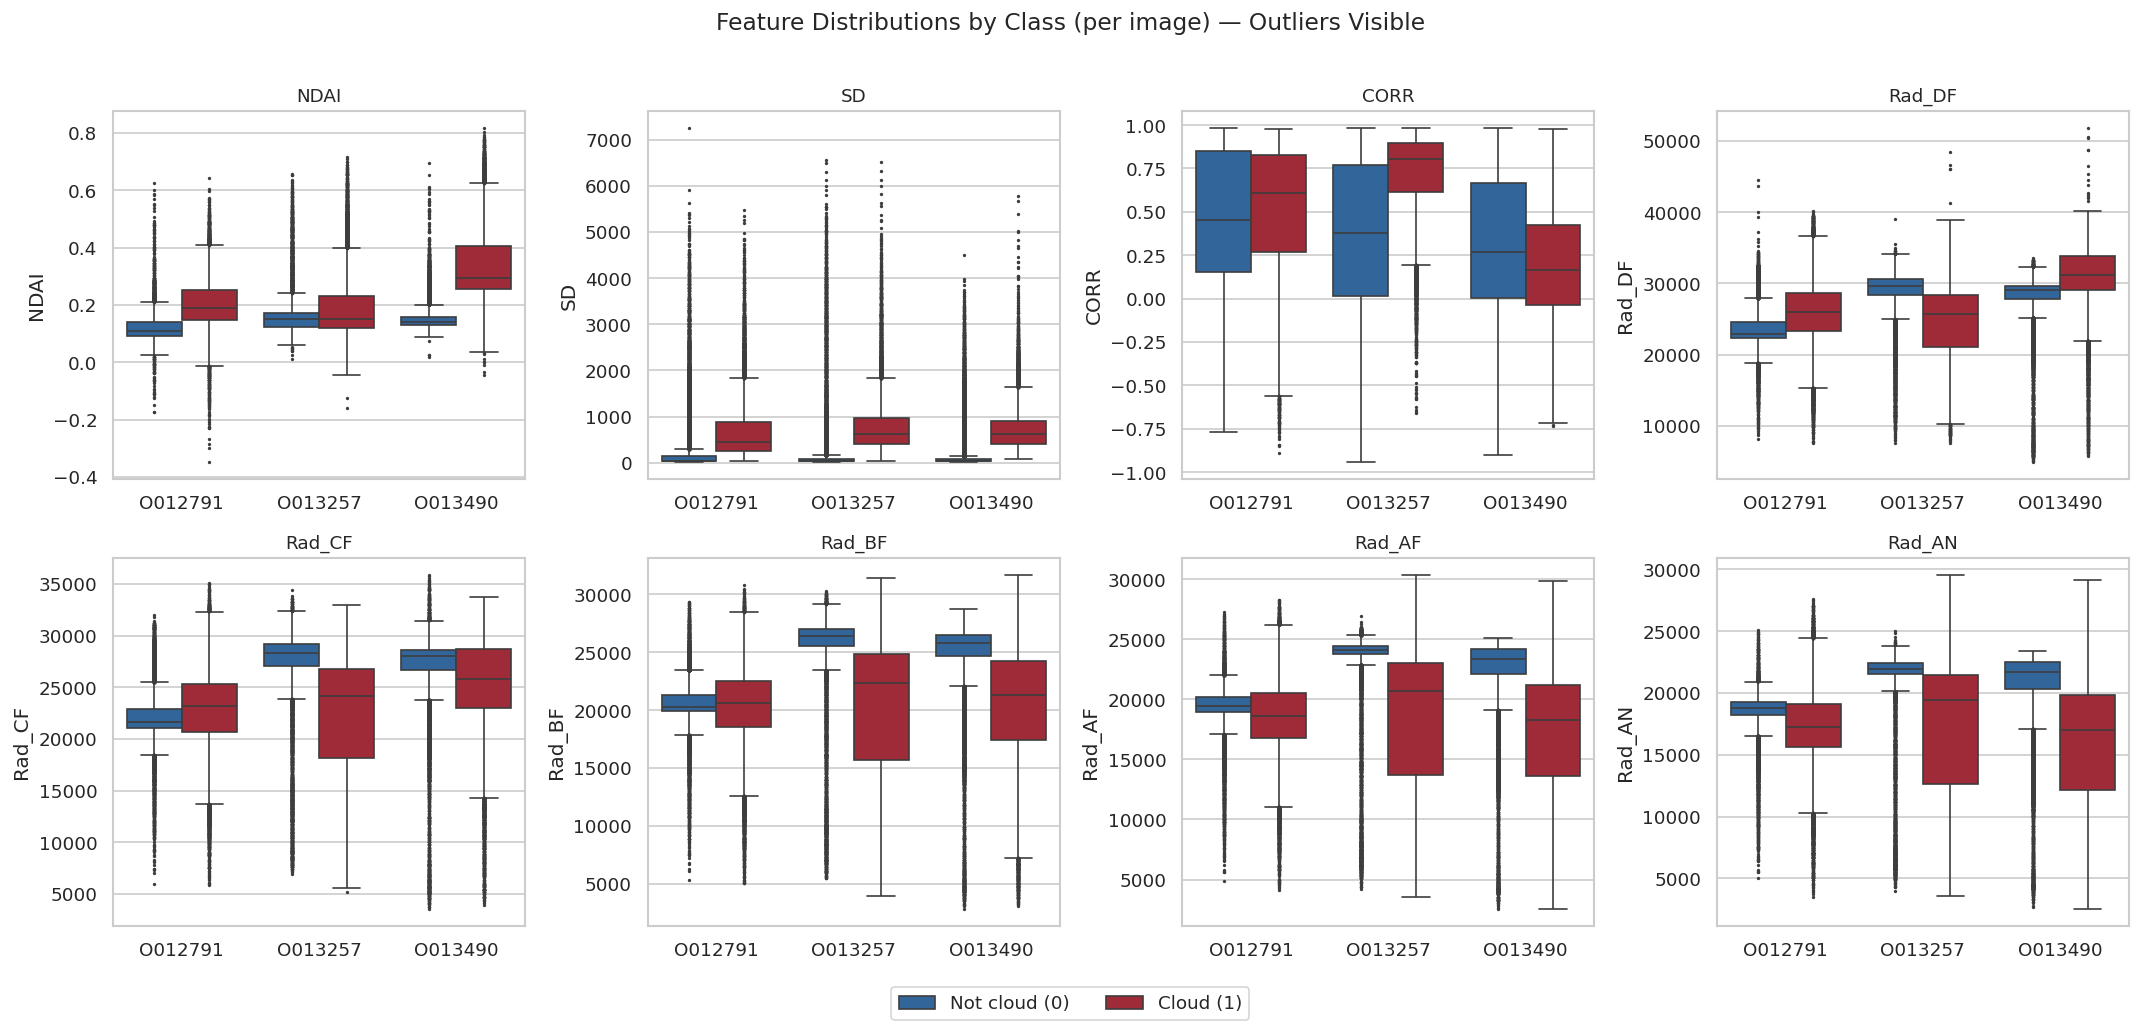
\includegraphics[width=1.00\textwidth]{./figures/feature_boxplots.png}
    \caption{Feature Boxplots by Cloud Label/Image}
    \label{fig:feat_boxplots}
\end{figure}
\FloatBarrier

From the above distributions, we observe a few characteristics. The first is that many of the variables do have differences between cloud classes that seem to be significant. For example, we see that cloudy pixels tend to have larger values for SD than non-cloud pixels. We also observe that there are differences between images. Looking at the CORR variable, we see that the first 2 images have higher values of CORR for cloudy pixels, whereas the opposite is true for the third image.

Looking at the radiance measurements, we see class distinctions across all measurements, with the mean difference in magnitude varying based on the image.

\begin{figure}[!htbp]
    \centering
    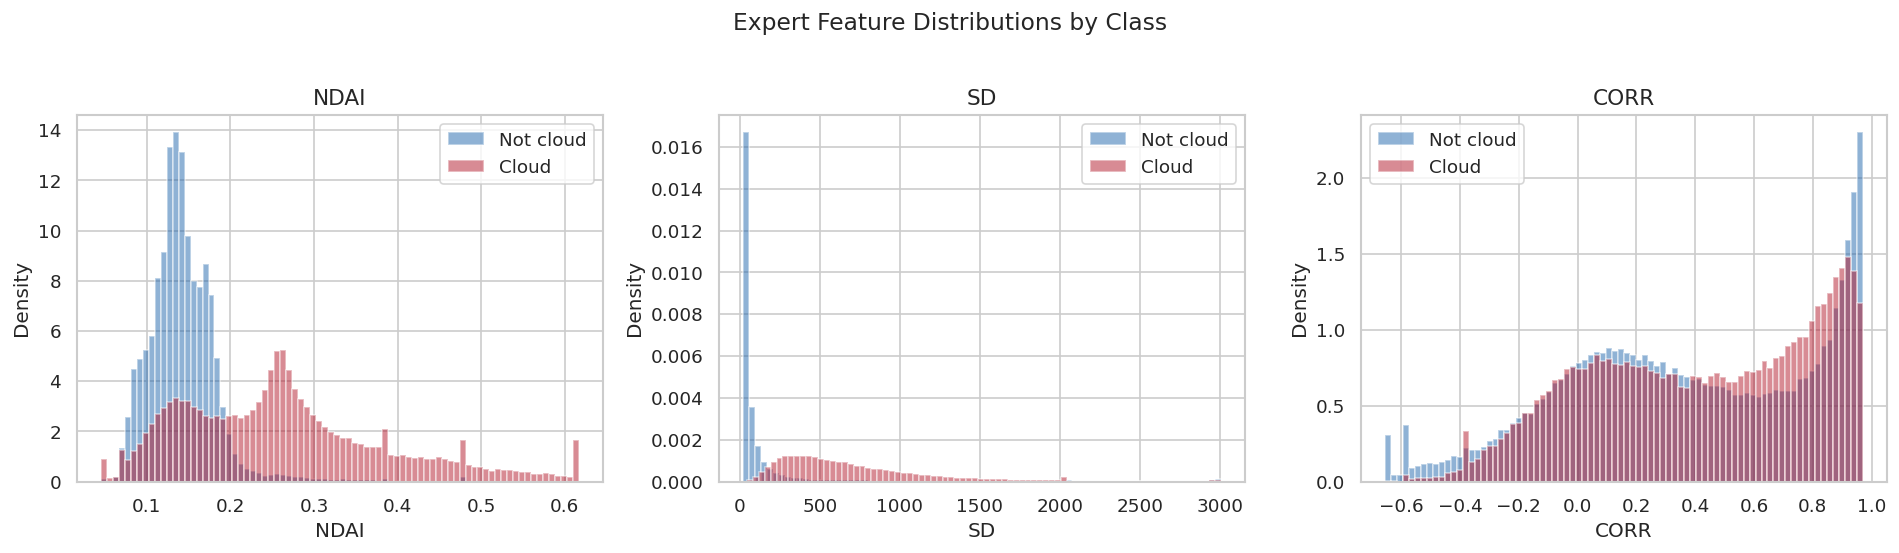
\includegraphics[width=1.00\textwidth]{./figures/expert_feature_histograms}
    \caption{Expert Feature Histograms by Cloud Label (All Images)}
    \label{fig:exp_feat_hists}
\end{figure}
\FloatBarrier

Figure \ref{fig:exp_feat_hists} presents histograms of the expert-derived features, aggregated for all three images. These figures more clearly indicate each features' individual ability to distinguish between clouds. NDAI and SD clearly show different distributions between cloud labels, with the cloudy pixels tending to have higher values of NDAI and a heavier tail for SD.

\begin{figure}[!htbp]
    \centering
    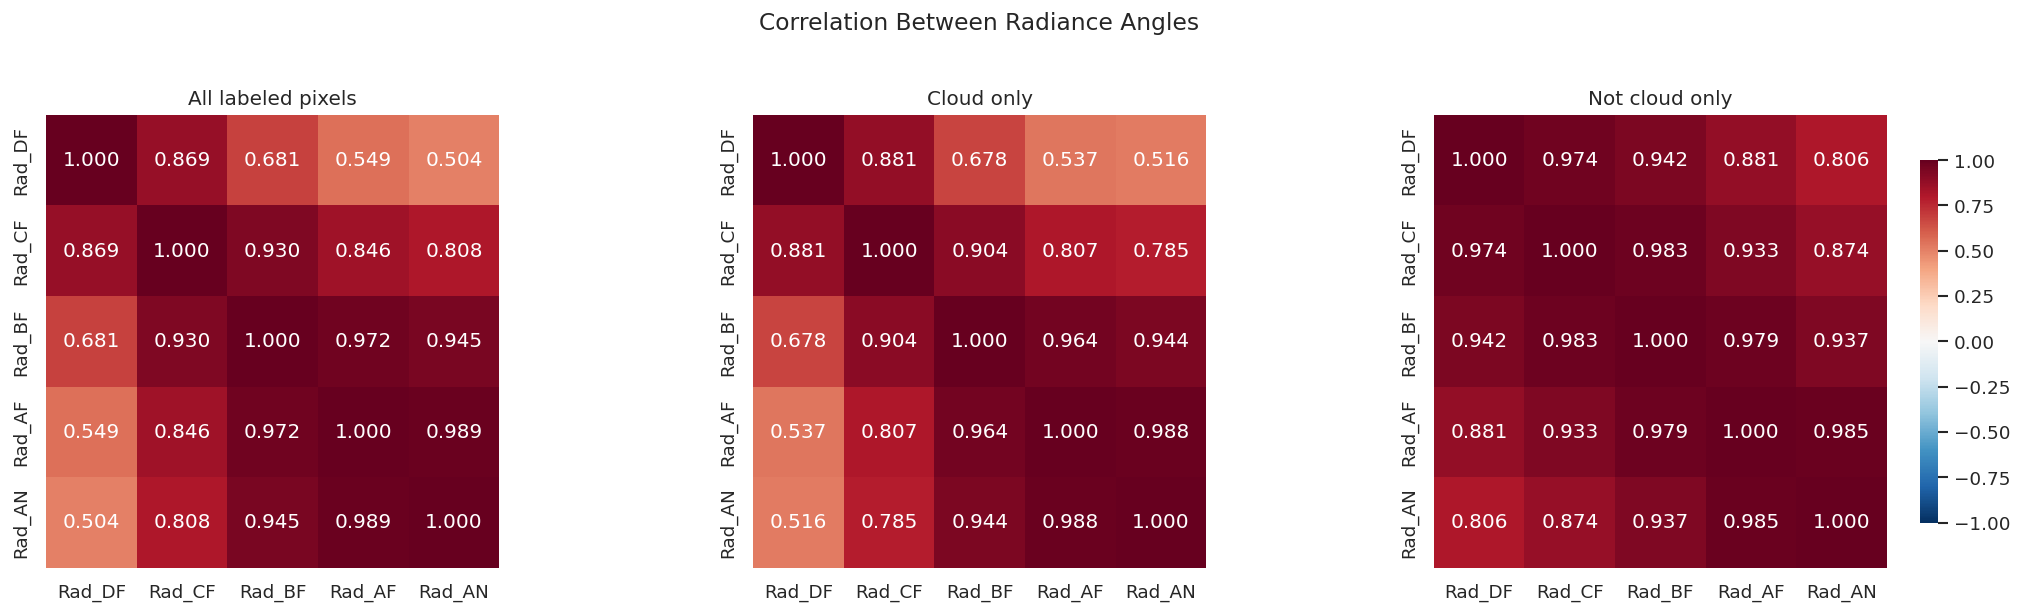
\includegraphics[width=1.00\textwidth]{./figures/cloud_no_cloud_correlations.png}
    \caption{Correlation Heatmaps of Radiance Measurements, Separated by Cloud/No Cloud Class}
    \label{fig:cloud_corr}
\end{figure}
\FloatBarrier

We also analyzed the correlations between radiance measurements separated by cloud/no cloud. We see that overall, there is high correlation among the radiance measurements but that the correlation is even higher among non-cloudy pixels. This phenomenon is explained by the scattering of radiation measurements mentioned in Shi et al. When radiation measurements are taken over a cloud-free surface, the correlations are expected to be high, whereas cloudy surfaces (especially clouds at a higher altitude) are expected to have lower correlations in radiation measurements \cite{Shi}.


\subsection{Data Splitting Strategy}

In this section, we outline how we split our data for training-testing for our predictive models. The way we split our data is an especially important choice because an improper split may lead to data leakage. For example, randomly assigning pixels to either the training/validation/testing set will introduce data leakage due to the spatial dependence of the features. To mitigate this, we introduce a \textbf{3-split image-level cross-validation}: in each split, two images will be used for training/validation (with an internal 80/20 stratified split) and one will act as the hold-out test set.

\begin{table}[h!]
\centering
\label{tab:cv_design}
\begin{tabular}{cccc}
\toprule
Split & Train (80\% + 20\% val) & Train images & Test \\
\midrule
1 & O013257 + O013490 & 122,328 pixels & O012791 \\
2 & O013490 + O012791 & 109,484 pixels & O013257 \\
3 & O012791 + O013257 & 100,479 pixels & O013490 \\
\bottomrule
\end{tabular}
\caption{Three-split image-level cross-validation design.}
\end{table}
\FloatBarrier

Within each split, we use 80\% of the training pixels to perform model fitting and 20\% to select the otpimal threshold for maximizing the F1-score. All hyperparameters are fixed a priori. The test images are never seen during the training phase, so there is no spatial leakage.

By splitting the data in this way, we are building $4 \text{ models/split}\times 3 \text{ splits} = 12$ models. In Section \ref{sec:model}, we analyze each model's performance across the different splits to reveal insights into the difficulties each model encountered when predicting on different images. This methodology also allows us to observe the effect of different images on model training and prediction. As we saw before, the images themselves have distributions of features that are not identical. They also have cloud coverages that vary widely, and in future images, it's possible for clouds to cover anywhere from 0\%-100\% of an image. This makes it difficult to build a generalizable, robust, and deployable model, as we only have three labeled images that don't fully represent the set of images we can train on, so by creating our splits like this, we observe the effect that our choice of training images has on modeling.

\subsection{Data Cleaning}

As part of our EDA, we performed the following validation checks on the labeled pixels:

\begin{itemize}
    \item No duplicate or missing pixels
    \item No missing values in the features
    \item No invalid (negative) radiance values
    \item No correlations outside of $[-1, 1]$
\end{itemize}

Overall, the dataset appears to already be rather clean, but we noticed many outlier values when analyzing the boxplots and histograms. These can present a problem during the modeling phase because they can have a high influence on the model. To resolve this, we performed winsorization on the data, which involves clipping the data to be at least the 1st percentile and at most the 99th percentile. This will still retain the overall distribution shape while reducing the impact of extreme outliers.

\section{Feature Engineering}
\label{sec:feat_eng}

\subsection{Most Informative Features}

To determine which features could best determine the presence of clouds, we used three metrics:

\begin{enumerate}
\item Pearson correlation with clouds
\item Random Forest feature importance using Gini impurity decrease
\item Permutation feature importance using a Random Forest
\end{enumerate}

We decided to use the correlation first for its simplicity, and we follow up with the feature importance and permutation importance to provide additional stability toward our conclusion of which variables are the best predictors. For the random forest we use default parameters for simplicity.

\begin{figure}[!htbp]
    \centering
    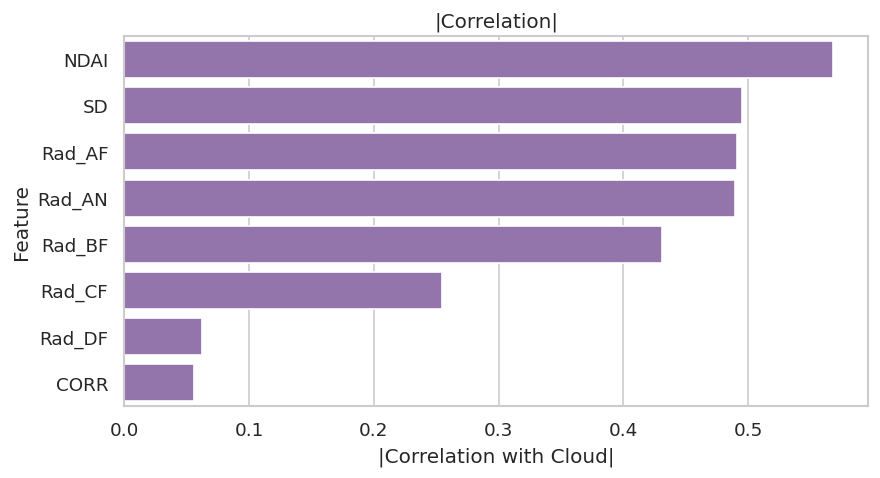
\includegraphics[width=1.00\textwidth]{./figures/feature_importance_corr.png}
    \caption{Feature Importance Using Correlation}
    \label{fig:feat_imp}
\end{figure}
\FloatBarrier

From Figure \ref{fig:feat_imp}, we see that the top three features with the strongest correlation with clouds appear to be NDAI, SD and RAD\_AF. However, we also provide some alternative viewpoints for which features may be important.

\subsubsection{Stability Check}

To analyze the stability of our findings, we decided to use mean decrease in impurity (MDI) and permutation importance from a random forest model as alternative metrics for feature importance. For the MDI, we trained a random forest model on the training data of Split 1. For the permutation importance plot, we used the validation set of Split 1 and computed the mean decrease in accuracy using 10 permutations of the feature.

\begin{figure}[!htbp]
    \centering
    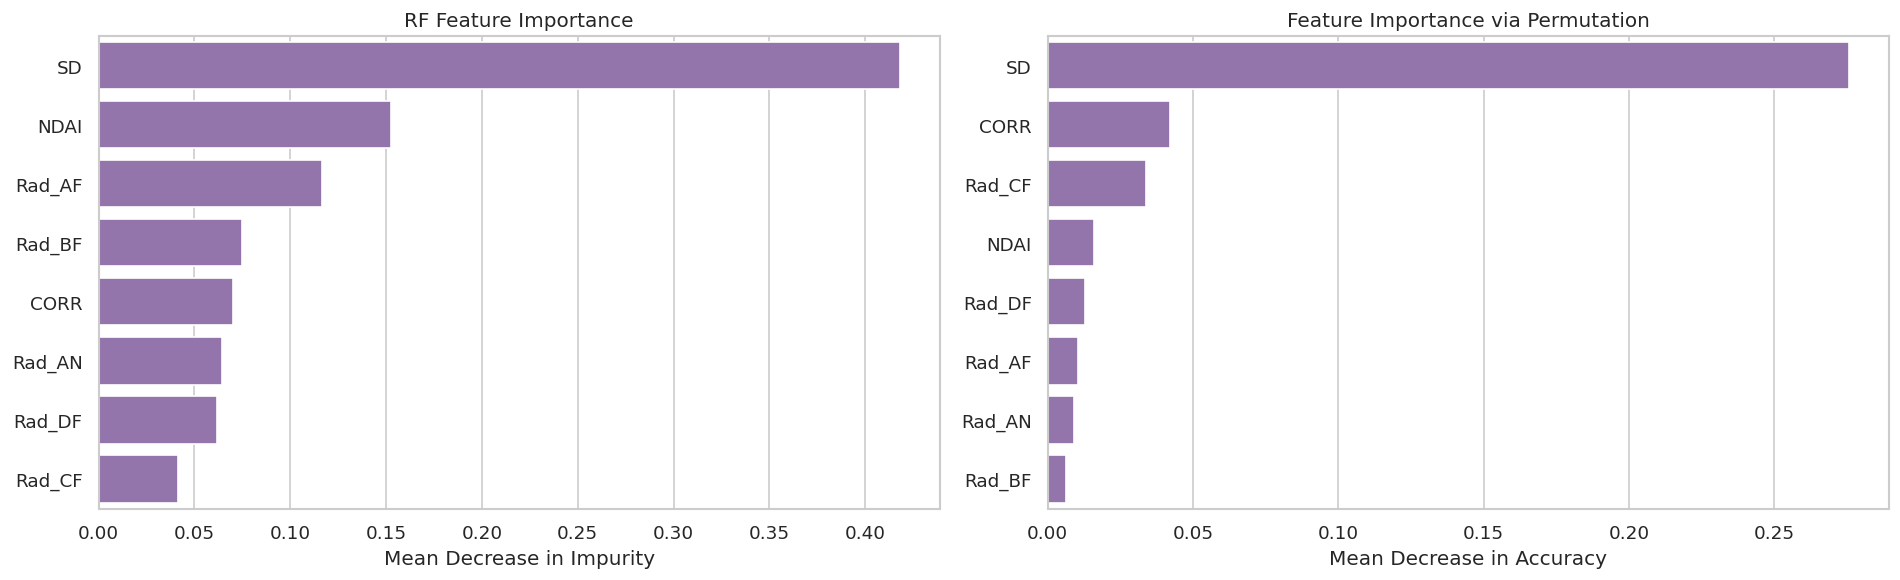
\includegraphics[width=0.9\textwidth]{./figures/feature_importance.png}
    \caption{Feature Importance Using Different Metrics}
    \label{fig:feat_imp_stable}
\end{figure}
\FloatBarrier

When we consider alternative metrics for measuring importance, we see some interesting results. From before, we observed that NDAI and SD seemed to be strong predictors, but CORR appeared to be weak. Its correlation with clouds appeared to be rather low. The left plot shows the MDI for the given features. From here, we see that CORR is no longer the least important predictor. This is likely because the random forest model was capable of capturing nonlinear trends and interactions that the correlation calculation could not. As another metric for identifying important features, we also analyzed the permutation importance plot when the random forest model was tested against the validation dataset. Interestingly, CORR now appears to be the second-most important variable, indicating that we shouldn't discount CORR's predictive power. SD's predictive power still appears to be very strong across the two metrics, while NDAI also appears to still be in the top four.

\subsubsection{Reality Check}

As another point of evidence toward CORR's predictive power, we look toward the enhanced linear correlation matching (ELCM) algorithm developed by Shi et al. As part of their predictive algorithm, they had the condition that a pixel was labeled non-cloudy when

\begin{itemize}
    \item $\text{SD}_{\text{AN}} < \text{threshold}_{\text{SD}}$ or
    \item $\text{CORR} > \text{threshold}_{\text{CORR}}$ and $\text{NDAI} < \text{threshold}_{\text{NDAI}}$ \cite{Shi}
\end{itemize}

The second condition in the algorithm indicates that CORR alone is not a strong predictor, and that it depends on NDAI to be able to discern clouds vs non-clouds. Furthermore, they elaborate that "degradation of detector performance is due mainly to the difference in the NDAI distributions between different visits" \cite{Shi}.

\subsection{Designing New Features}

Given the information for our EDA, as well as the domain knowledge provided in Shi et al., we decided to engineer a few different features.

\subsubsection{Correlation Improvement: Mean Squared Rank Difference}

From Figure \ref{fig:cloud_corr}, we observed that non-cloud regions tended to have extremely highly correlated radiance measurements across different camera angles, whereas cloud regions also had highly correlated radiance measurements, but not as severe, which aligns with the findings in Shi et al. \cite{Shi}. Also observing that CORR's isolated predictive power was rather weak, we tried to engineer our own CORR feature, where low values would correspond to highly correlated measurements across camera, and high values would correspond to more weakly correlated radiance measurements. To do so, we assigned a rank to each radiance measurement and computed the variance of ranks across the five radiance measurements. Thus, similarly ranked measurements would produce a small value, whereas more weakly correlated ranks would produce a larger value.

\subsubsection{Pooling Mean Squared Rank Differences}

One limitation of the previous feature is that it doesn't consider the correlation with surrounding patches. To account for this, we observed $9\times 9$ patches of pixels and calculated the variance in mean squared rank difference for each patch of pixels. We also experimented with patches of size $5 \times 5$ and $3 \times 3$ and found that the $9 \times 9$ patches were better able to discriminate between clouds and non-clouds.

\subsubsection{Pooling Other Variables}

Further iterating on this idea of looking at patches of data, we decided to calculate the mean and standard deviation of the NDAI, SD, and CORR variables across $15 \times 15$ and $9 \times 9$ patches. Similar to before, we observed that overall, larger patch sizes tended to be more effective at capturing the spatial structure, but we expect that there is a point for which the patch size is too large and will smooth out significant signals.

\subsubsection{Logarithmic Transforms}

We also applied the transformation $g(x) = \log(1+\max(x, 0))$ to SD and each of the radiation measurements. The reason for doing so is this can make these variables more approximately normally distributed, which would be useful for any inference we conduct in a regression.

\subsubsection{Pairwise Interactions}

We also create pairwise interactions between NDAI, CORR, $\log(1+\text{SD})$. The goal for doing so is that we hope that the predictive models that we employ in the next section can capture non-linear boundaries between these variables. We applied the log transform to the SD variable to make its distribution more approximately normal.

\subsubsection{Angular Anisotropy Indices}

For each of the four angles, we calculated a normalized difference between the radiance measurement at that angle and the radiance measurement of the nadir angle, which we call the angular anisotropy index. In doing so, we hope to provide another attempt at directly encoding the angular dependence of radiance, which can be useful for distinguishing between clouds and non-clouds.

$$
\text{aniso}_j=\frac{\text{Rad}_j-\text{Rad}_{\text{AN}}}{\text{Rad}_j+\text{Rad}_{\text{AN}}}
$$

\subsubsection{Adjacent-Angle Radiance Ratios}

We also computed the ratio between consecutive angular channels:

$$
\text{ratio}_{j, j+1}=\frac{\text{Rad}_j}{\text{Rad}_{j+1}}
$$

This provides another mechanism for capturing the angular dependence between radiance measurements, which may be useful for distinguishing between clouds and non-clouds, as it captures local gradients in the angular radiance profile.

\subsubsection{Sobel Gradient}

Building upon the ideas discussed above regarding pooling and taking gradients, we decided to take the Sobel gradient of the original features. The Sobel gradient is used in image processing for edge detection, acting as a high-pass filter that can sharpen edges between boundaries \cite{Gonzalez}. By sharpening the boundaries, we hope that a predictive model can better discern between the cloud and non-cloud regions.

\subsubsection{Preliminary Results}

Figure \ref{fig:top_10_feat_eng} shows the top 10 features after engineering. Overall, we see that many of our strategies appear to be effective in capturing the distinction between clouds and non-clouds. In particular, taking the log transform of the SD variable significantly increases its original correlation from 0.49 to 0.76. The interaction between NDAI and $\log(\text{SD})$ also appears to be significant. Looking at both $15 \times 15$ and $9 \times 9$ patches of these variables also shows an improvement in correlation.

\begin{figure}[!htbp]
    \centering
    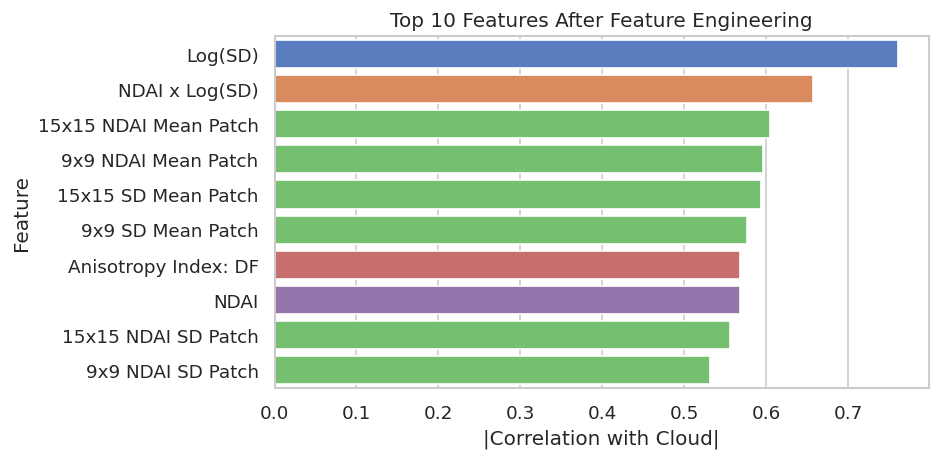
\includegraphics[width=0.75\textwidth]{./figures/feature_engineering_top_10.png}
    \caption{Results of Feature Engineering Colored by Feature Type: Blue = Log Transform, Orange = Interaction, Green = Spatial, Red = Anisotropy Index, Purple = Expert}
    \label{fig:top_10_feat_eng}
\end{figure}
\FloatBarrier

Additionally, we saw an improvement in the CORR variable's isolated ability to distinguish between clouds. CORR originally presented a correlation of 0.056 across all images for clouds. When we took the mean-squared rank difference, this correlation increased to 0.154, and we observed a further improvement when we pooled this metric in $9 \times 9$ patches of pixels, increasing its correlation to 0.378. The other transformations saw some minor improvements for some features, whereas for others, they were not able to significantly improve the correlation of that feature.

\subsection{Transfer Learning}

Transfer learning is a machine learning technique where a model that is trained on one task is applied to another task. In our case, we have 161 unlabeled images that we want to leverage, so we will apply transfer learning to use these images for our cloud prediction models. To accomplish this, we constructed an autoencoder, implemented via Pytorch Lightning, that performs feature extraction and dimensionality reduction on the unlabeled images, and use these features as predictors in our predictive models. In that regard, the autoencoder acts as a nonlinear generalization of PCA.

We first modified the architecture of the baseline autoencoder to instead be a \textbf{convolutional} autoencoder, which took advantage of the 2D spatial structure of the data, rather than discarding it. As we observed from our feature engineering work, features that looked at patches of data tended to be more effective than features that looked at an individual pixel because they captured the spatial structure of the data. To utilize this finding, we modified the architecture to scan through $9 \times 9$ patches of pixels instead of flattening them. The encoder uses three convolutional layers to reduce the dimension of the input layers down to $5 \times 5$, applying batch normalization to accelerate and stabilize the training, and using the ReLU activation function to capture the nonlinearity of the data between each layer. Once the encoder has reduced the dimension down to the desired embedding size, the decoder (whose structure mirrors the encoder) projects the embedded feature space back to the size of the original input space.

After deciding on an architecture, we then conducted a two-stage hyperparameter sweep to select the optimal hyperparameters that minimized the validation MSE. Stage 1 was a random search over 12 configurations spanning embedding dimensions (8, 16, 32), learning rates $(10^{-4}\text{ to }10^{-3})$, Gaussian noise injection for regularization $(\sigma=0 \text{ to } 0.2)$, and random channel masking for regularization $(p = 0 \text{ to } 0.25)$. This stage identified that an embedding dimension of 32 and learning rate of $10^{-3}$ was clearly dominant. All configurations with these settings achieved a validation MSE $< 0.10$, while smaller embeddings or lower learning rates stalled above 0.13. In Stage 2, we conducted a targeted grid search over noise and masking levels within the best region, which confirmed that the simplest configuration (no noise, no masking) achieves the lowest validation MSE of 0.0909. After training, we extract the 32-dimensional embeddings for every pixel by passing its local $9 \times 9$ neighborhood through the autoencoder.

\begin{table}[h!]
\centering
\label{tab:ae_sweep}
\small
\begin{tabular}{ccccccl}
\toprule
Embed & LR & Noise $\sigma$ & Mask $p$ & Val MSE & Train MSE & Stage \\
\midrule
\textbf{32} & \textbf{0.001} & \textbf{0.0} & \textbf{0.0} & \textbf{0.0909} & \textbf{0.0897} & 2 \\
32 & 0.001 & 0.0 & 0.0 & 0.0915 & 0.0906 & 2 \\
32 & 0.001 & 0.1 & 0.0 & 0.0918 & 0.0905 & 2 \\
32 & 0.001 & 0.2 & 0.0 & 0.0920 & 0.0909 & 2 \\
32 & 0.001 & 0.0 & 0.15 & 0.0939 & 0.1061 & 2 \\
32 & 0.001 & 0.1 & 0.15 & 0.0945 & 0.1089 & 2 \\
32 & 0.001 & 0.2 & 0.15 & 0.0951 & 0.1111 & 2 \\
32 & 0.0005 & 0.05 & 0.1 & 0.0971 & 0.1063 & 1 \\
32 & 0.001 & 0.2 & 0.25 & 0.1010 & 0.1257 & 2 \\
\midrule
16 & 0.0001 & 0.2 & 0.0 & 0.1390 & 0.1396 & 1 \\
16 & 0.0001 & 0.0 & 0.1 & 0.1430 & 0.1534 & 1 \\
8 & 0.001 & 0.2 & 0.0 & 0.1644 & 0.1623 & 1 \\
8 & 0.0001 & 0.2 & 0.0 & 0.1787 & 0.1747 & 1 \\
8 & 0.0001 & 0.2 & 0.25 & 0.1821 & 0.2011 & 1 \\
\bottomrule
\end{tabular}
\caption{Two-stage autoencoder hyperparameter sweep (19 runs total, sorted by val MSE). Stage~1: random search over a broad grid. Stage~2: targeted grid search around the best region (embed=32, lr=0.001).}
\end{table}

\newpage

These embeddings capture spatial patterns that complement the pixel-level features provided and the features we engineered. In Section \ref{sec:model}, we will see that while our engineered features were effective in capturing trends not original in the pixel-level data, the autoencoder also captured useful features that we did not anticipate.

\section{Modeling}
\label{sec:model}

\subsection{Classification Models}

We trained four classifiers using scikit-learn on the data excluding the unlabeled pixels: logistic regression, random forest, gradient boosted trees (GBM), and k-nearest-neighbors (KNN).

\subsubsection{Logistic Regression}

A logistic regression model is a simple method for computing predictions. We assume that the log odds can be represented by a linear combination of the features:

$$
\ln\left(\frac{p}{1-p}\right)=\beta_0+\beta_1x_1 + \dots + \beta_kx_k
$$

From our EDA and feature engineering, we observed that many of the raw features exhibited nonlinear relationships with the label. However, our feature engineering and feature extraction capture these nonlinear relationships to the best of our ability.

Our implementation using scikit-learn uses the \texttt{class\_weight} parameter set to \texttt{"balanced"}, which penalizes the misclassifications of the minority class. For example, if the image is mostly clouds, we wan to to prioritize correctly labeling non-cloud pixels. It applies a weight that is inversely proportional to class frequencies using the following formula:

$$
    w_i = \frac{n}{2\cdot n_i} \quad \text{for} \quad i\in \{0, 1\}
$$

\subsubsection{Random Forest (RF)}

A random forest builds trees in parallel. Our implentation using scikit learn using 250 trees with \texttt{min\_samples\_leaf} set to 2. This means that we will never create a new leaf in a tree if that leaf would only have a single observation in it. Additionally, we have set the \texttt{class\_weight} to \texttt{"balanced\_subsample"}. In doing so, each tree in the random forest is trained on a bootstrapped sample, with the class weights computed using the same formula as in Logistic Regression. However, it is computed once for each tree, as each tree sees a different subsample of the data.

\subsubsection{Gradient Boosted Trees (GBM)}

A modification on pure random forests that sequentially trains ``weak learners." Unlike Random Forests, which build the trees in parallel, GBT's build a tree in sequence. Our implementation in scikit learn uses the same \texttt{min\_samples\_leaf} as our RF implementation, along with the default \texttt{learning\_rate} and \texttt{n\_estimators} of 0.1 and 100 respectively. These are there to specify the weight given to new predictions when ``boosting" and the number of trees to aggregate to our sequentially generated final tree. We chose to set \texttt{max\_depth} (the number of nodes in each tree) to 5, and \texttt{subsample} (the percent of the total sample to use when generating a tree) to $80\%$. The latter will reduce our overall variance, but at the cost of increased bias.

\subsubsection{$k$-Nearest Neighbors (KNN)}

$k$-Nearest Neighbors works by looking at the $k$ data points closest to a point and assigning it as cloud or no-cloud based on a voting of those $k$ points. For our implementation, we opted to use "weighted" voting, where closer points had a larger influence on the vote. KNN assumes that points that are "close" exhibit similar characteristics and thus share the same label. We use the $\ell_2$ norm over the $\ell_1$ norm as our distance metric because we are not working with count data, for which we would typically use the $\ell_1$ norm \cite{Yu}.

The KNN algorithm also assumes that all of the features operate on the same scale. This is not true for our dataset, so we perform SD-scaling before running the algorithm. We opted to use $k=15$ because we believed that it provided a moderate amount of smoothing against label noise while still preserving local decision boundaries.

\subsection{Cross-Validation Results}

We initially measure the performance of these four models in our 3-fold cross validation using the following metrics, still excluding unlabeled pixels:
\vspace{10pt}

\renewcommand{\arraystretch}{1.3}
\begin{tabular}{l p{10cm}}
\textbf{Metric} & \textbf{Description} \\
\hline
$\text{Precision} = \frac{\text{TP}}{\text{TP} + \text{FP}}$ 
& The fraction of predicted clouds that are correctly labeled. \\

$\text{Recall} = \frac{\text{TP}}{\text{TP} + \text{FN}}$ 
& The fraction of actual clouds that were correctly labeled. \\

$\text{F1} = \frac{2 \cdot \text{Precision} \times \text{Recall}}{\text{Precision} + \text{Recall}}$ 
& Harmonic mean of precision and recall. \\

$\text{Balanced Accuracy} = \frac{\text{TPR} + \text{TNR}}{2}$  
& The arithmetic mean of the true positive and true negative rates. \\

ROC-AUC 
& The area under the curve in the model's ROC plot. \\

PR-AUC 
& The area under the curve in the model's Precision-Recall plot.
\end{tabular}
\vspace{10pt}

A precision recall curve is similar to a receiver operator characteristic curve, except we are plotting recall against precision instead of FPR against TPR. Table~\ref{tab:cv_results} presents the main results.

\begin{table}[H]
\centering
\small
\begin{tabular}{lcccccc}
\toprule
Model & Precision & Recall & F1 & Bal.\ Acc. & ROC-AUC & PR-AUC \\
\midrule
\textbf{Logistic Reg.} 
& 0.839$\pm$0.119 
& 0.889$\pm$0.101 
& \textbf{0.856$\pm$0.087} 
& 0.898$\pm$0.060 
& 0.962$\pm$0.026 
& 0.918$\pm$0.057 \\

Random Forest 
& 0.923$\pm$0.084 
& 0.727$\pm$0.203 
& 0.792$\pm$0.139 
& 0.835$\pm$0.088 
& 0.950$\pm$0.051 
& 0.932$\pm$0.058 \\

GBM 
& 0.928$\pm$0.064 
& 0.766$\pm$0.215 
& 0.819$\pm$0.140 
& 0.862$\pm$0.095 
& \textbf{0.973$\pm$0.023} 
& \textbf{0.941$\pm$0.047} \\

KNN 
& 0.849$\pm$0.119 
& 0.744$\pm$0.151 
& 0.782$\pm$0.114 
& 0.826$\pm$0.085 
& 0.893$\pm$0.065 
& 0.817$\pm$0.117 \\
\bottomrule
\end{tabular}
\caption{3-fold cross-validation results (test set). Mean $\pm$ std across folds.}
\label{tab:cv_results}
\end{table}

Notice that Logistic Regression achieves the highest mean F1 (0.856). However, the GBM leads in ROC-AUC (0.973) and PR-AUC (0.941). The standard deviations are quite large in many cases, which reflects the difficulty in generalizing across images with different cloud patterns.

\subsection{Per-Split Breakdown}

Let's focus in on the F1 score and compare the results of the different models on our different splits instead of looking at the mean over all three. 

\begin{figure}[H]
\centering
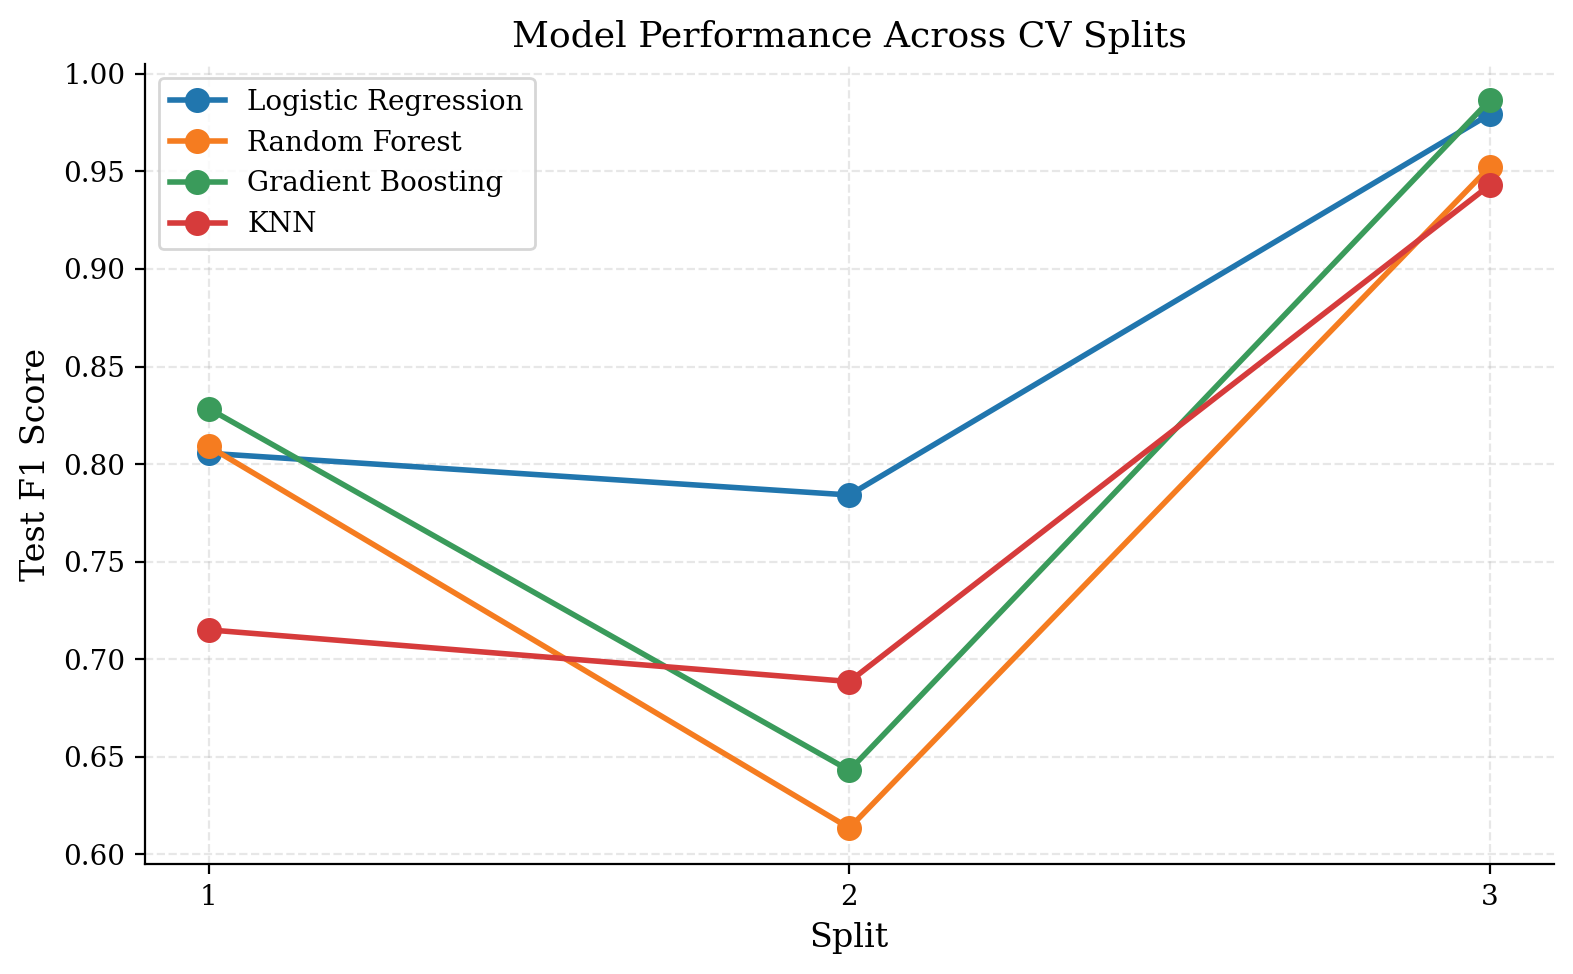
\includegraphics[width=0.7\textwidth]{figures/cv_fold_comparison.png}
\caption{Per-split test F1 for each model. All models perform best on split~3 (O013490) and worst on split~2 (O013257).}
\label{fig:cv_folds}
\end{figure}

The image used for the test set in Split 2 (O013257) has the lowest cloud fraction (17.8\% from Table~\ref{table:cloud_coverage}) and a slightly different cloud shape, making it the hardest image to predict. Below are the prediction maps for our four models on splits 2 and 3: the hardest and the easiest.

\begin{figure}[H]
\centering

\includegraphics[width=\textwidth]{figures/fold_2/spatial_predictions.png}
\caption{Ground truth and model predictions for Split~2 test image (O013257): red = cloud, blue = no cloud. This is the hardest split due to low cloud fraction and distribution shift.}
\label{fig:spatial_fold2}
\end{figure}

\begin{figure}[H]
\centering

\includegraphics[width=\textwidth]{figures/fold_3/spatial_predictions.png}
\caption{Ground truth and model predictions for Split~3 test image (O013490): red = cloud, blue = no cloud. All models perform well on this split.}
\label{fig:spatial_fold3}
\end{figure}

\newpage

Lastly, let's look at the precision and recall performance over the three splits:

\begin{table}[H]
\centering
\small
\begin{tabular}{lcccccc}
\toprule
& \multicolumn{3}{c}{Precision} & \multicolumn{3}{c}{Recall} \\
\cmidrule(lr){2-4} \cmidrule(lr){5-7}
Model & Split 1 & Split 2 & Split 3 & Split 1 & Split 2 & Split 3 \\
\midrule
LogReg & 0.868 & 0.681 & 0.969 & 0.751 & 0.924 & 0.990 \\
RF & 0.804 & 0.978 & 0.987 & 0.814 & 0.447 & 0.921 \\
GBM & 0.838 & 0.970 & 0.975 & 0.819 & 0.481 & 0.998 \\
KNN & 0.684 & 0.902 & 0.960 & 0.749 & 0.557 & 0.927 \\
\bottomrule
\end{tabular}
\caption{Per-split precision and recall, revealing different failure modes across models and splits.}
\label{tab:perfold_detail}
\end{table}


We can see in Table~\ref{tab:perfold_detail} that the different models express different struggles with precision and recall. Notice that, in split 2, GBM has high precision (0.970), but very low recall (0.481), meaning it misses most clouds rather than hallucinating them. On the other hand, logistic regression takes the opposite approach. It has lower precision (0.681), but much higher recall (0.924), meaning it catches more clouds at the cost of more false positives. So, depending on the use case, we may prefer one model over another.



\subsection{Detailed Split 1 Diagnostics}

Since split 1 (test = O012791) represents the moderately difficult case, let's focus in on it and look at some detailed diagnostics.
Figure~\ref{fig:roc_pr_fold1} shows ROC and PR curves mentioned in Table~\ref{tab:cv_results}. The GBM and logistic regression dominate in area under both curves. The shape of the precision-recall curve for KNN indicates that KNN has trouble maintaining precision at reasonable recall levels.

\begin{figure}[H]
\centering
\begin{subfigure}[t]{0.48\textwidth}
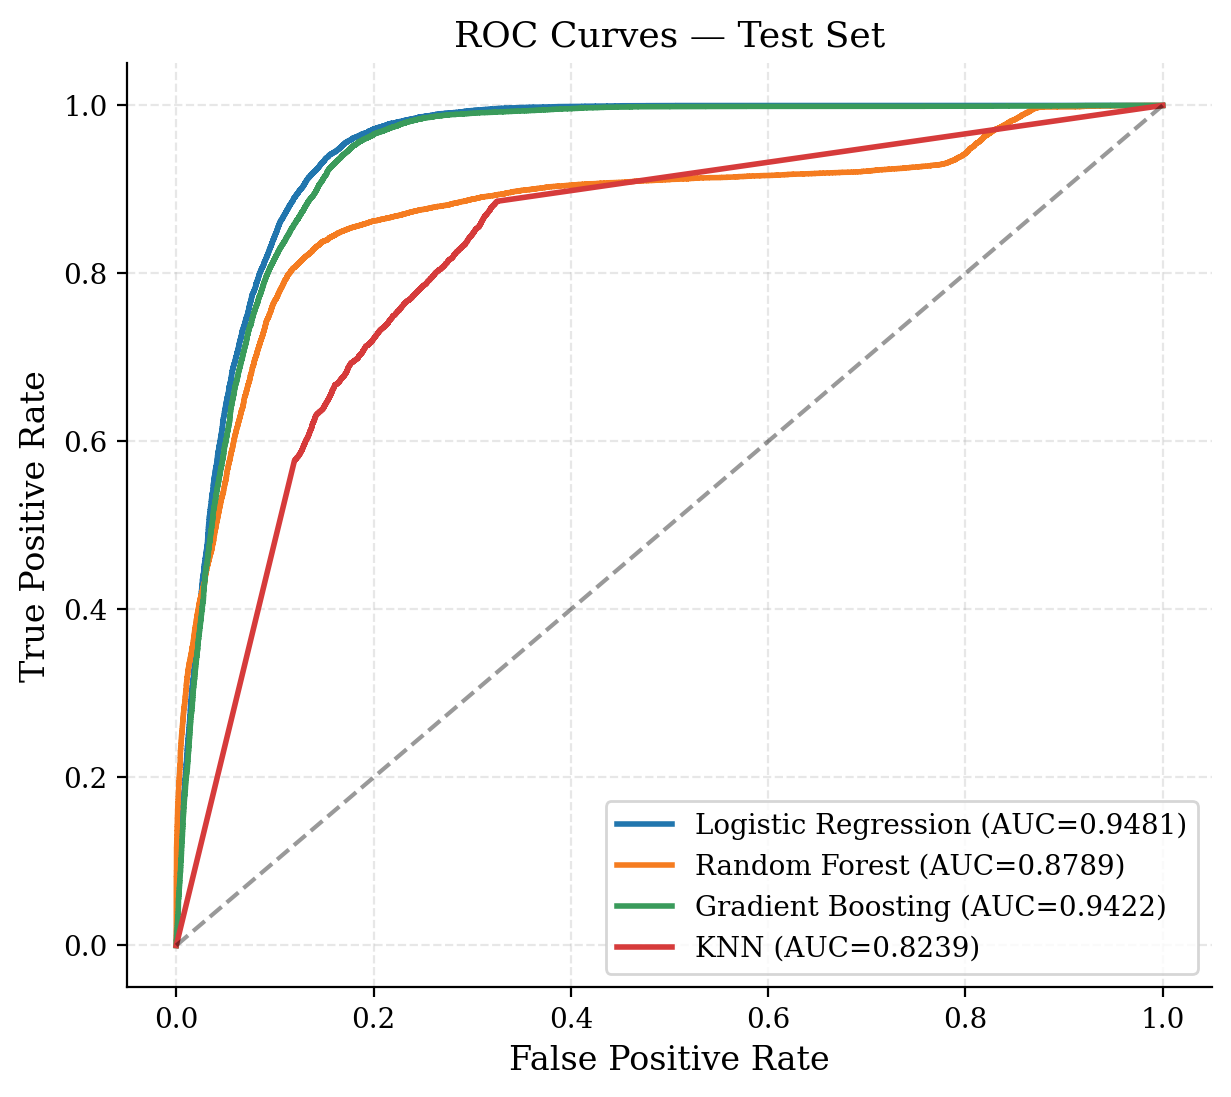
\includegraphics[width=\textwidth]{figures/fold_1/roc_curves.png}
\caption{ROC curves.}
\end{subfigure}
\hfill
\begin{subfigure}[t]{0.48\textwidth}
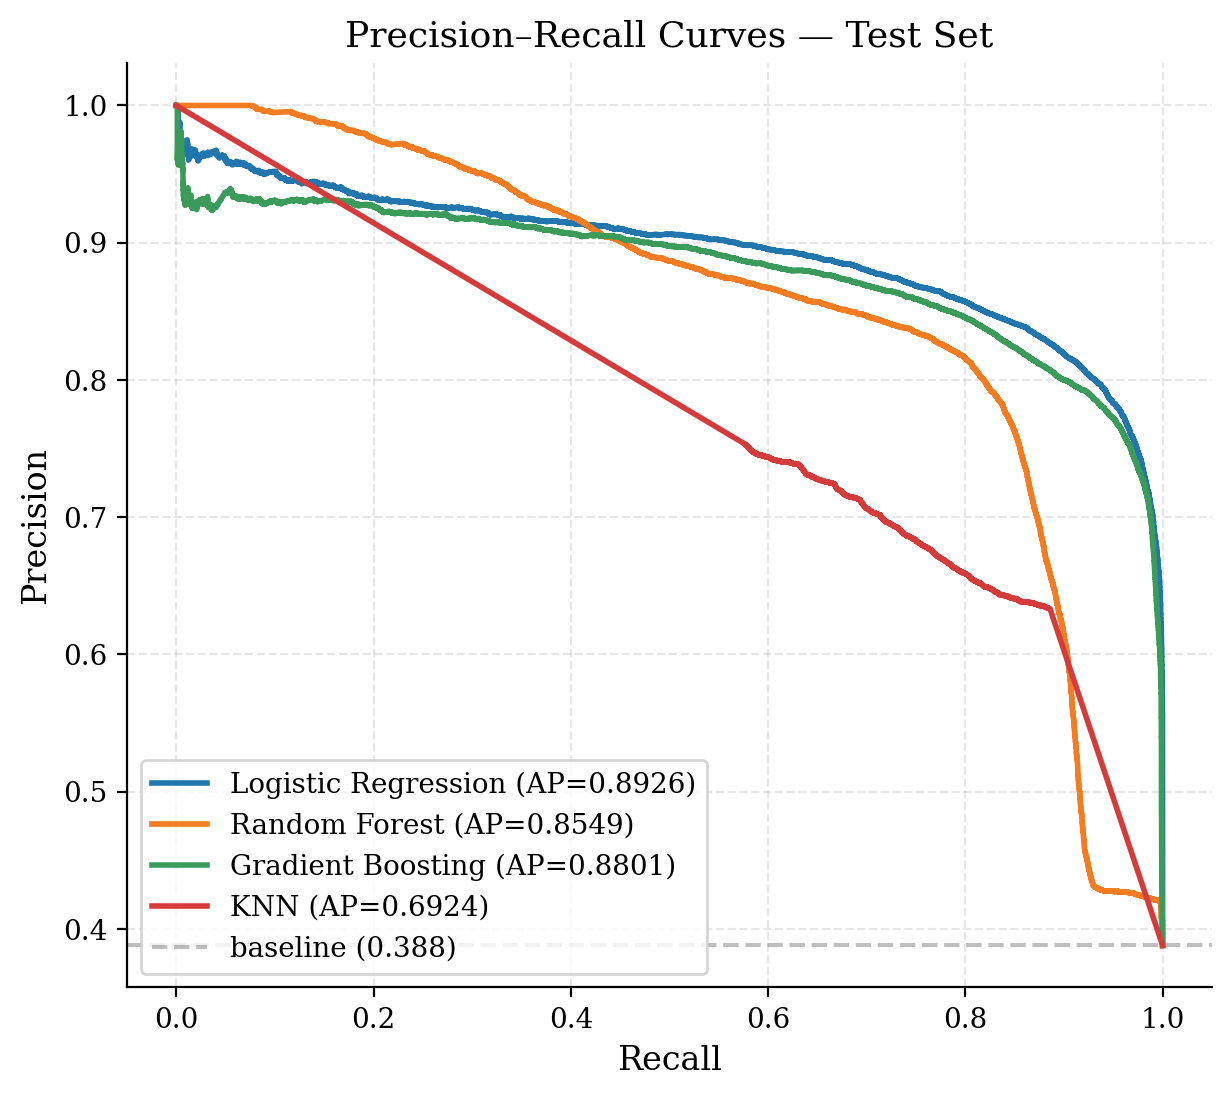
\includegraphics[width=\textwidth]{figures/fold_1/pr_curves.png}
\caption{Precision-Recall curves.}
\end{subfigure}
\caption{ROC and PR curves for Split~1 (test: O012791). GBM and logistic regression achieve the highest AUC values.}
\label{fig:roc_pr_fold1}
\end{figure}

Figure~\ref{fig:cm_fold1} shows the confusion matrices for all four models on Split~1. This matches our analysis from Table~\ref{tab:perfold_detail}. We can again see that the different models trade off false positives and false negatives in different ways.

\begin{figure}[H]
\centering
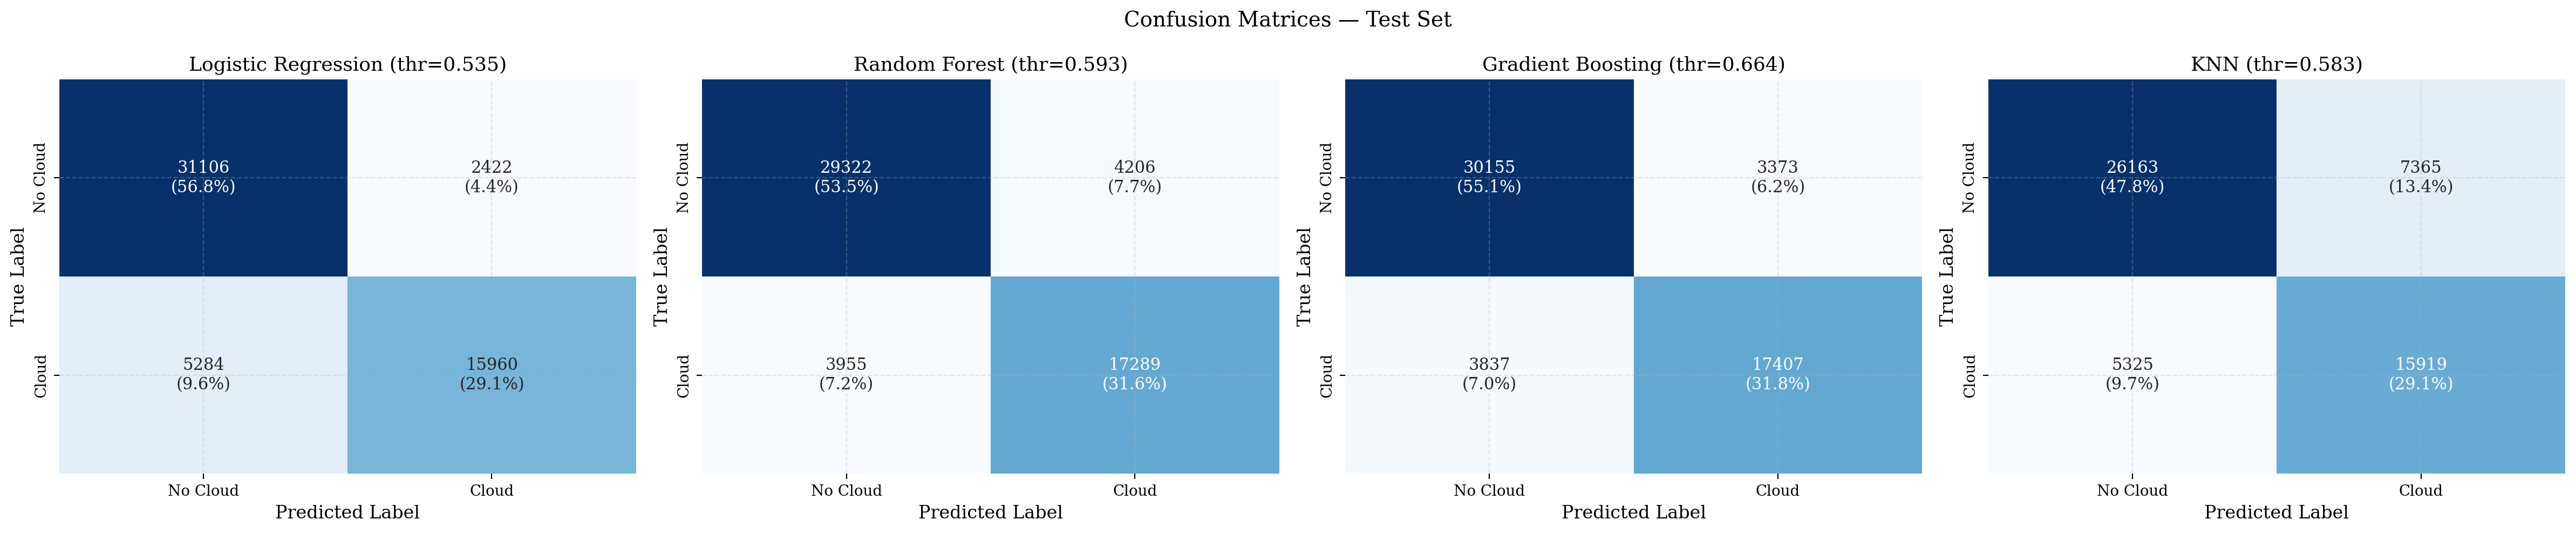
\includegraphics[width=\textwidth]{figures/fold_1/confusion_matrices.png}
\caption{Confusion matrices for Split~1 test set (O012791). Each matrix: TN (top-left), FP (top-right), FN (bottom-left), TP (bottom-right).}
\label{fig:cm_fold1}
\end{figure}

\subsection{Best Model Selection}

Ultimately, we choose \textbf{logistic regression} as our primary model. It achieves the highest mean F1 ($0.856 \pm 0.087$, from Table~\ref{tab:cv_results}). Now, GBM has higher ROC-AUC (0.973 vs.\ 0.962, also from Table~\ref{tab:cv_results}), but with only 3 folds this difference is not statistically meaningful. Additionally, we use F1 instead of AUC to select the model because AUC only measures ranking quality, not the actual classification output. A model with perfect AUC can still produce poor cloud predictions. Lastly, logistic regression is more consistent in it's F1 metric across splits (std = 0.087 vs.\ 0.140 for GBM, from Table~\ref{tab:cv_results}), and it's coefficients can be read directly. When higher precision is needed (0.928 vs.\ 0.839, from Table~\ref{tab:cv_results}), GBM can be used instead.

\subsection{Post-Hoc Analysis}

\subsubsection{Feature Selection}

Continuing to use Split~1 as a reference, let's take a moment to look how the model metrics feed into our choice of features. First, by plotting the random forest Gini importance and logistic regression coefficient magnitudes, sorted by Gini importance.

\begin{figure}[H]
\centering
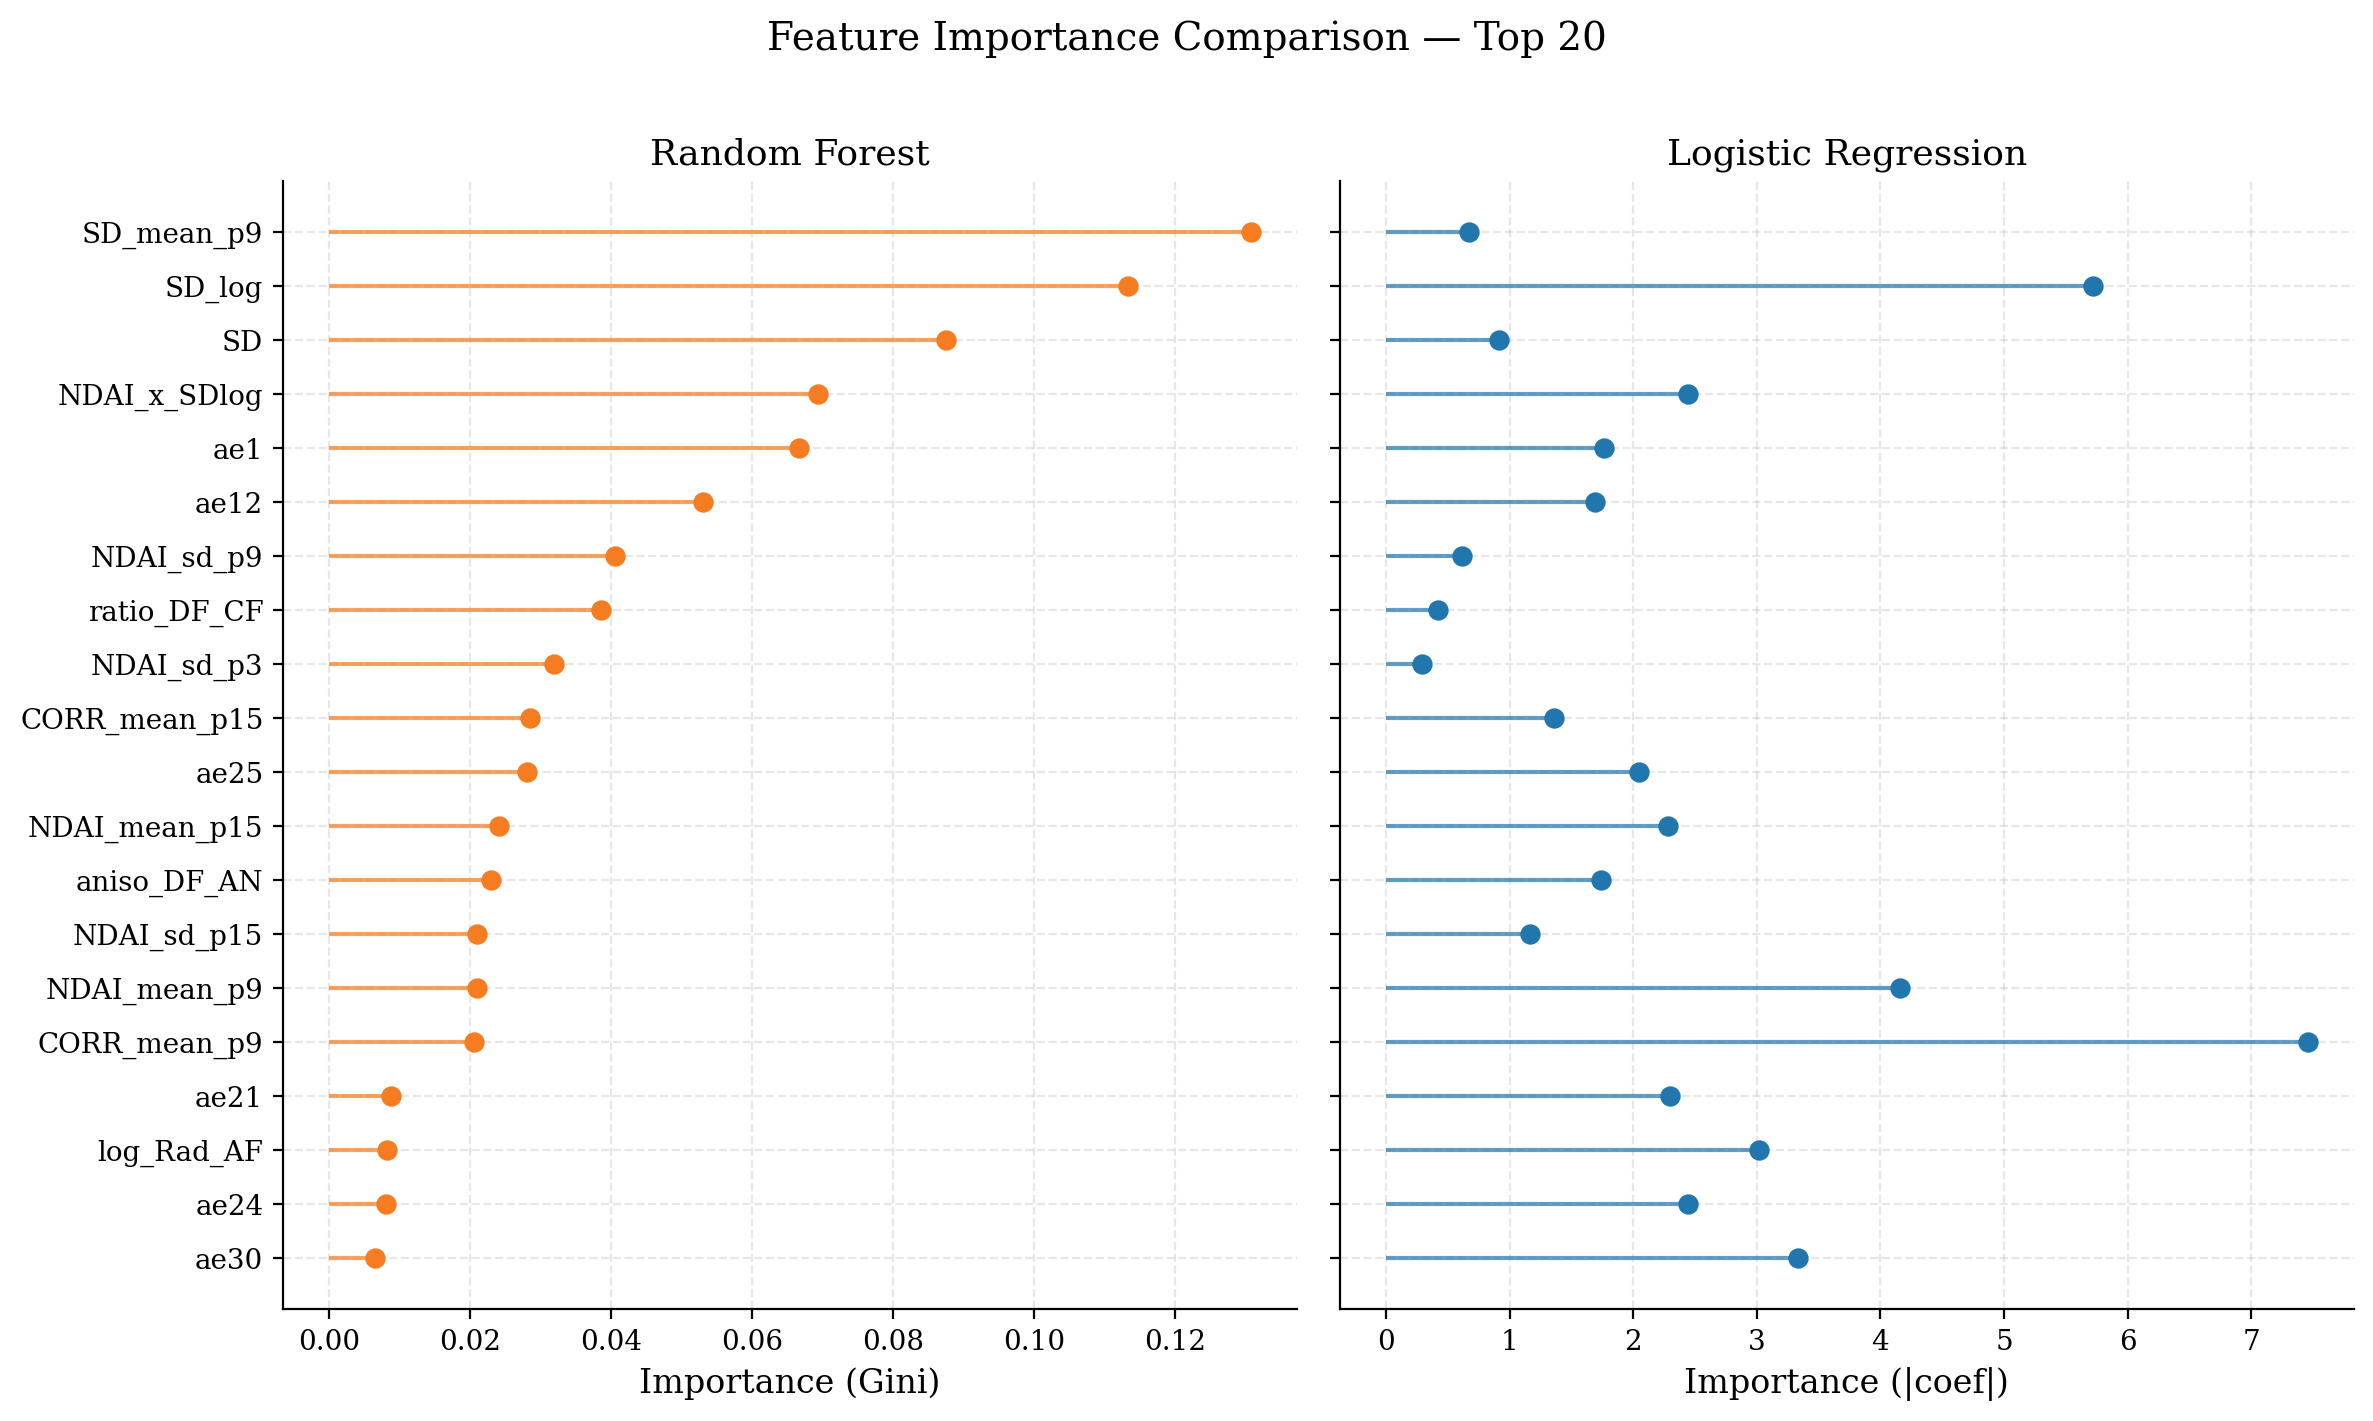
\includegraphics[width=0.7\textwidth]{figures/fold_1/feature_importance_combined.png}
\caption{Top-20 features ranked by Random Forest Gini importance (left) and logistic regression absolute coefficients (right), Split~1.}
\label{fig:feat_importance}
\end{figure}

We can see that, for the RF model, features that are related to the standard deviation have the largest impact. On the other hand, logistic regression puts a lot of weight on features we engineered to aggregate over $9\times 9$ patches (\texttt{CORR\_mean\_p9} and \texttt{NDAI\_mean\_p9}) as well as our $\log$ transformed standard deviation (\texttt{SD\_log}). In order to perform a similar analysis using the GBM model, we used Shapley Additive Explanation (SHAP) values.

SHAP values quantify the contribution of each feature to a single prediction by modeling the prediction process as a cooperative game, where features act as players. Each feature’s contribution is computed as its average marginal effect across all possible subsets of features. In Figure~\ref{fig:shap}, we plot the mean absolute SHAP values and a beeswarm plot that displays the shap value for each prediction by feature. For example, we can see that low values of \texttt{SD\_mean\_p9} (the blue points on the bottom row of the beeswarm plot) correspond to a large negative impact on the prediction generated by the model in most cases. In fact, the importance of \texttt{SD\_mean\_p9} in the GBI model is the most legible result from Figure~\ref{fig:shap}.

\begin{figure}[H]
\centering
\begin{subfigure}[t]{0.48\textwidth}
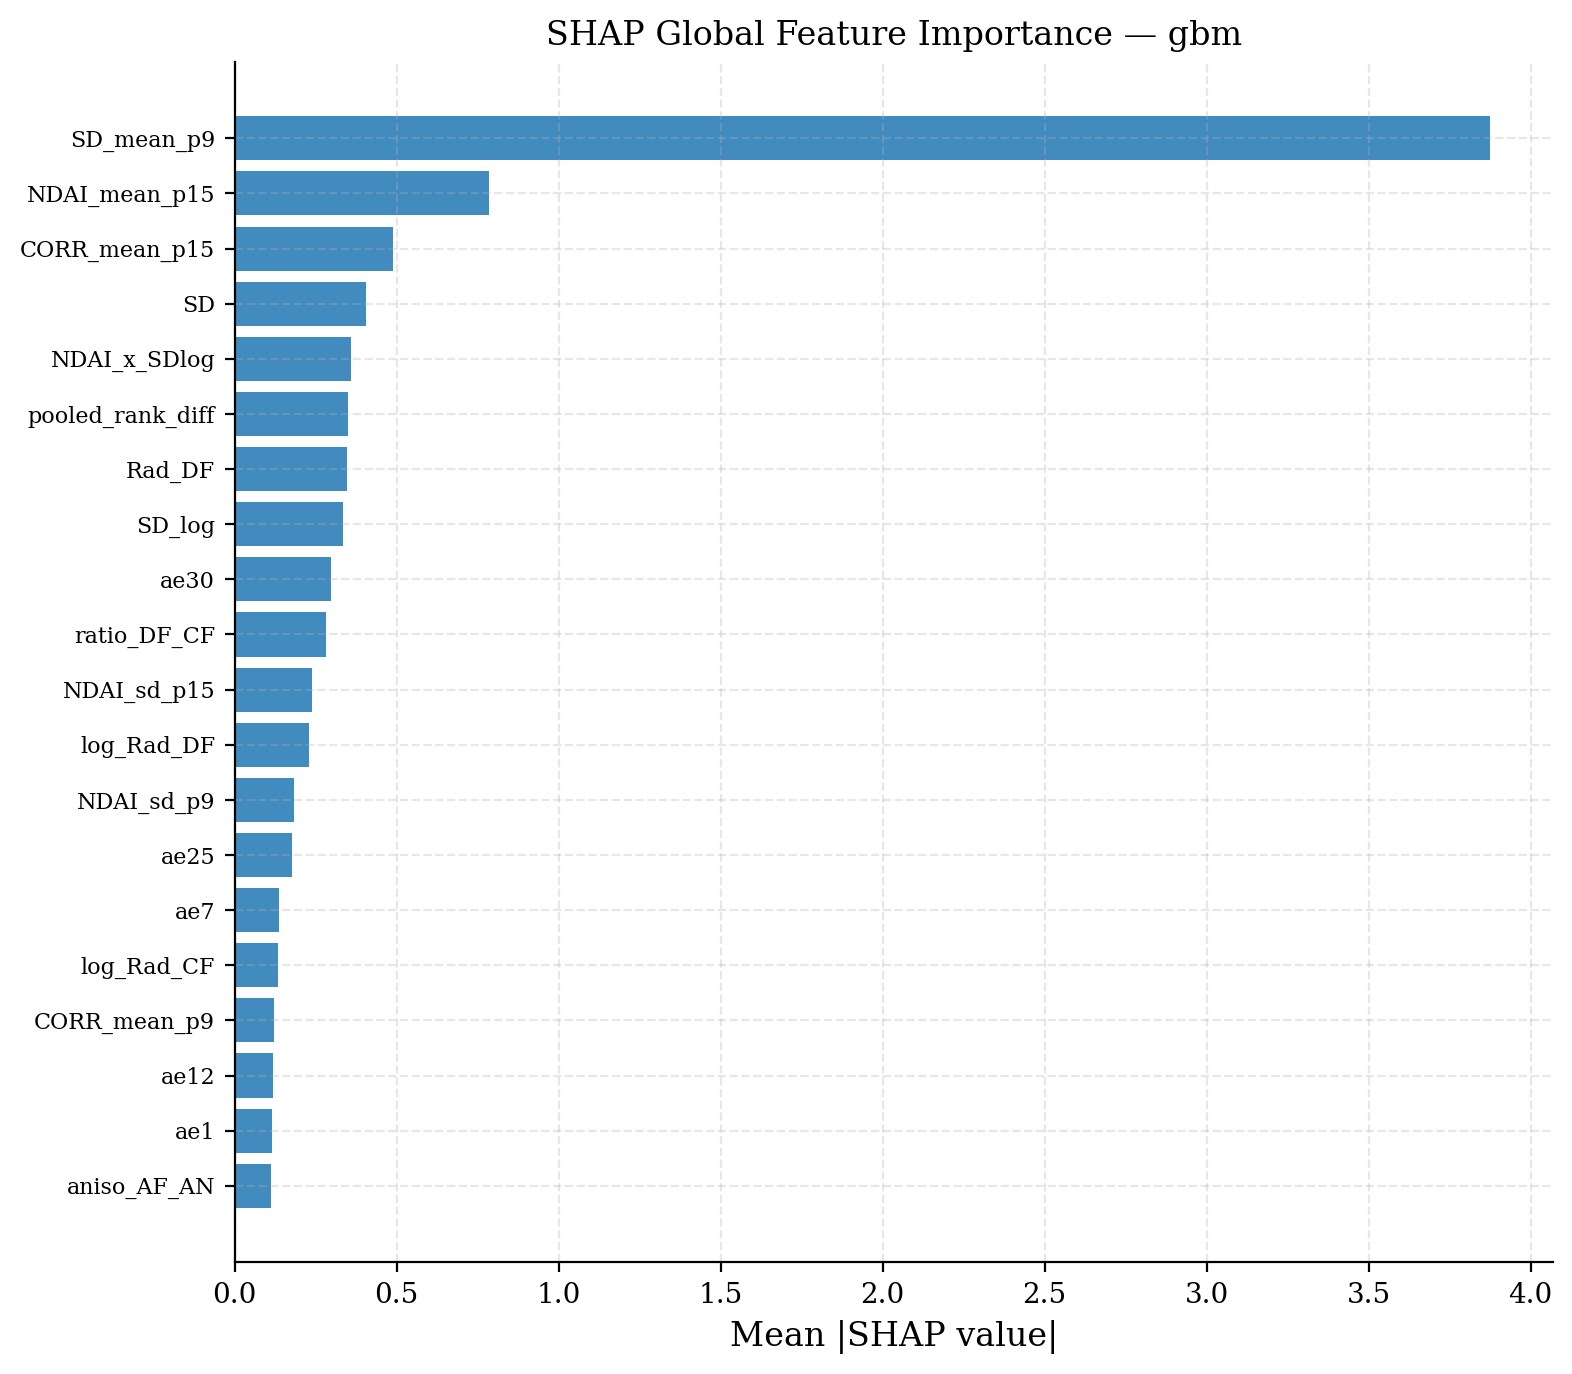
\includegraphics[width=\textwidth]{figures/fold_1/shap_bar_gbm.png}
\caption{Global importance (mean $|\text{SHAP}|$).}
\end{subfigure}
\hfill
\begin{subfigure}[t]{0.48\textwidth}
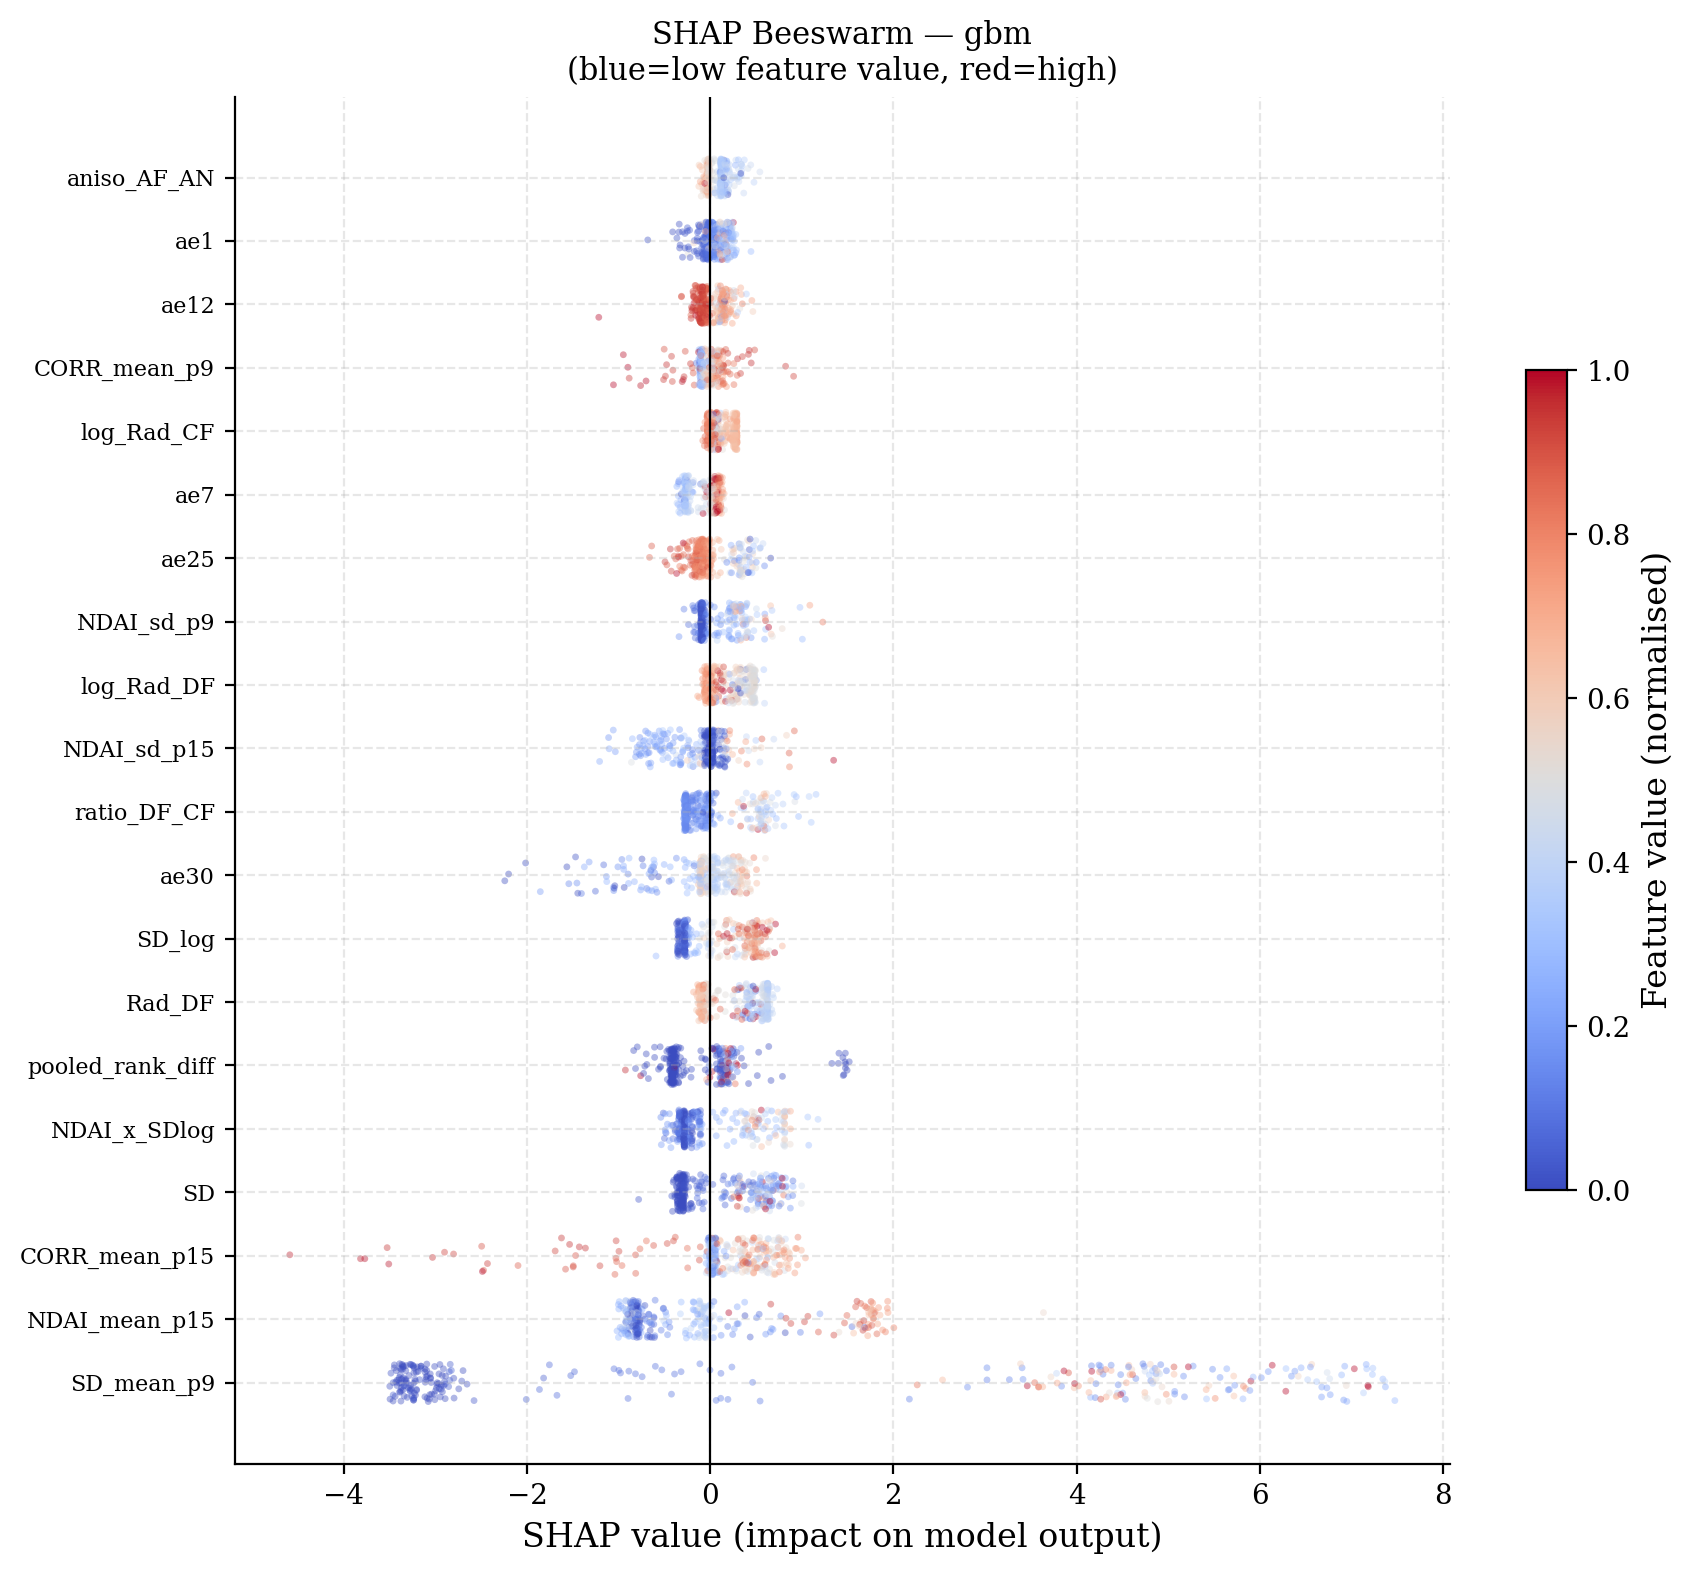
\includegraphics[width=\textwidth]{figures/fold_1/shap_beeswarm_gbm.png}
\caption{Beeswarm: color = feature value.}
\end{subfigure}
\caption{SHAP analysis for GBM (Split~1). Left: \texttt{SD\_mean\_p9} dominates global importance. Right: high SD spatial means push toward cloud, high CORR spatial means push toward non-cloud.}
\label{fig:shap}
\end{figure}

Another way we can check feature significance in our logistic regression model is with an ablation study, where we will start with a base set of features to evaluate the model on, then slowly add more to see the impact that the addition of features has on the performance of the model. The results are below:

\begin{table}[H]
\centering
\begin{tabular}{lcccc}
\toprule
Feature Set & \# Features & F1 & PR-AUC & ROC-AUC \\
\midrule
Expert (NDAI, SD, CORR) & 3 & 0.743$\pm$0.161 & 0.736$\pm$0.132 & 0.846$\pm$0.112 \\
Radiance (5 channels) & 5 & 0.654$\pm$0.207 & 0.750$\pm$0.160 & 0.773$\pm$0.143 \\
Raw (expert + radiance) & 8 & 0.737$\pm$0.152 & 0.737$\pm$0.121 & 0.819$\pm$0.100 \\
Enhanced (no AE, no spatial) & 25 & 0.815$\pm$0.119 & 0.914$\pm$0.058 & 0.961$\pm$0.026 \\
Enhanced + AE (no spatial) & 57 & \textbf{0.866$\pm$0.089} & 0.907$\pm$0.070 & 0.956$\pm$0.032 \\
Enhanced (full) & 71 & 0.856$\pm$0.087 & \textbf{0.918$\pm$0.057} & \textbf{0.962$\pm$0.026} \\
\bottomrule
\end{tabular}
\caption{Feature ablation study using logistic regression (3-fold CV test, Mean $\pm$ std). Best mean value is bolded.}
\label{tab:ablation}
\end{table}

We can see that there is almost a net improvement by continuing to add features past the raw features we are given. Both in the sense of improved mean metrics, and lower standard deviations. However, The 71-feature space includes substantial redundancy: many spatial statistics are highly correlated with each other, and the 32 autoencoder dimensions likely capture overlapping information.

In order to ``cull the herd," we rank all features by their mean absolute SHAP value from the full GBM model (the top 20 are displayed in Figure~\ref{fig:shap}), then retrain GBM using only the top-$k$ features and evaluate via the same 3-fold CV. We can see the results in Table~\ref{tab:feat_select}.

\begin{table}[H]
\centering
\begin{tabular}{cccl}
\toprule
Features $k$ & Mean F1 & Mean ROC-AUC & Notes \\
\midrule
10 & 0.780 & 0.955 & \\
15 & 0.806 & 0.965 & \\
20 & 0.800 & 0.964 & \\
30 & 0.817 & 0.969 & $\approx$ full model \\
50 & 0.820 & 0.973 & \\
71 (all) & 0.819 & 0.973 & baseline \\
\bottomrule
\end{tabular}
\caption{Feature selection: GBM performance with top-$k$ SHAP features.}
\label{tab:feat_select}
\end{table}

Performance increases steeply from 10 to 30 features, then plateaus. With 30 features, GBM achieves F1 = 0.817 and ROC-AUC = 0.969, nearly identical to the full 71-feature model (0.819 and 0.973). At 50 features, F1 actually exceeds the full model (0.820 vs.\ 0.819), suggesting that the additional 21 features introduce mild noise. The top-5 features span three distinct families: \texttt{SD\_mean\_p9} (spatial texture), \texttt{CORR\_mean\_p15} (spatial coherence), \texttt{SD} (raw expert), \texttt{NDAI\_x\_SDlog} (engineered interaction), and \texttt{Rad\_DF} (raw radiance). Autoencoder embeddings (\texttt{ae30}, \texttt{ae25}, \texttt{ae12}) appear in positions 10-15. This demonstrates that expert variables, initial feature engineering, and autoencoder embeddings all contribute some non-redundant information. Lastly, we can demonstrate the importance of certain features with a Lasso Path plot (Figure~\ref{fig:lasso}).

\begin{figure}[H]
\centering
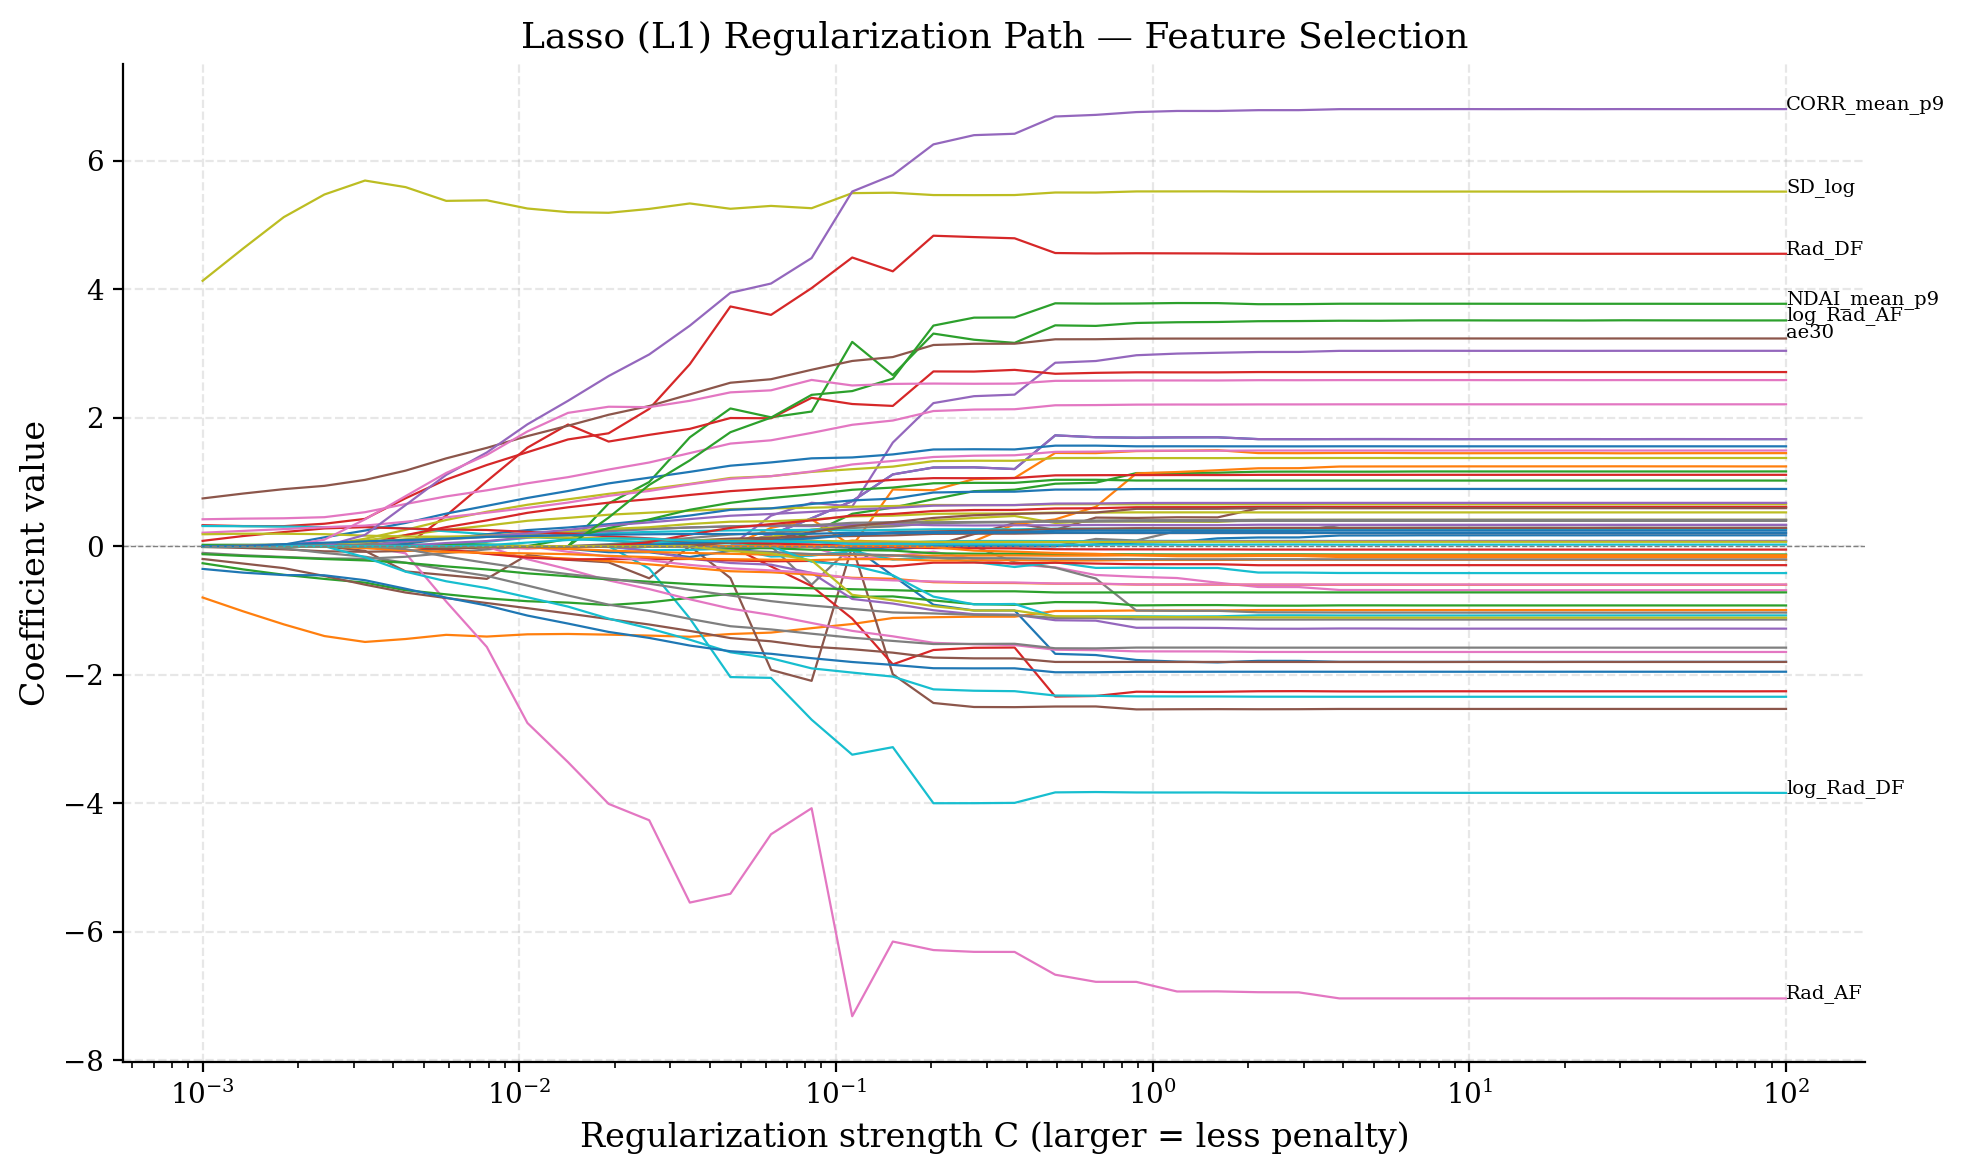
\includegraphics[width=0.7\textwidth]{figures/fold_1/lasso_path.png}
\caption{L1 regularization path for logistic regression. Each line traces a feature's coefficient as penalty decreases ($C$ increases). \texttt{CORR\_mean\_p9}, and \texttt{SD\_log} dominate early; many spatial features remain near zero, confirming redundancy.}
\label{fig:lasso}
\end{figure}

Notice how a variety of features display importance as the penalty starts to decrease. Features that rely on aggregating over nearby pixels (\texttt{CORR\_mean\_p9} and \texttt{NDAI\_mean\_p9}), some engineered features (\texttt{SD\_log} and \texttt{log\_Rad\_AF}), and some expert features (\texttt{Rad\_AF} and \texttt{Rad\_DF}).

\subsubsection{Adaptive Thresholding}
\label{sec:adaptive}

A typical approach to thresholding would tune a single decision threshold for the probability that a pixel is cloud on the validation set and apply it to all test images. This works when the validation and test distributions are similar, but breaks down when they differ. When using only the expert-labeled images given to us, the fixed threshold is tuned on training images with 29-48\% cloud fraction (excluding unlabeled pixels). However, it is then applied to a test image that may have very different cloud prevalence. When the test image has less cloud than expected, the threshold is too aggressive and produces excessive false positives (e.g., RF in Fold~2 with fixed threshold = 0.628 produces F1 = 0.613).

We propose to use Otsu's method for adaptive thresholding to determine when to label a pixel a cloud based on $\text{P(cloud)}$, instead of using the training-derived threshold. This is similar to the work done in Shi et al using QDA to adaptively threshold NDAI. \cite{Shi}. We apply Otsu's method to the predicted probability distribution of each test image independently. Otsu's method finds the threshold that maximizes the between-class variance of the probability histogram, effectively locating the natural split point between the cloud and non-cloud probability modes. This requires no labeled data when applied to the test set and adapts to the specific image the model is being tested on.

Our analysis showed that adaptive thresholding in this manner improved every model on average, with the largest gains on the hardest cases. This is shown in Table~\ref{tab:adaptive}.
 
\begin{table}[H]
\centering
\small
\begin{tabular}{lccccccc}
\toprule
& \multicolumn{3}{c}{Fixed Threshold F1} & \multicolumn{3}{c}{Adaptive Threshold F1} & \\
\cmidrule(lr){2-4} \cmidrule(lr){5-7}
Model & Split 1 & Split 2 & Split 3 & Split 1 & Split 2 & Split 3 & $\Delta$ Mean \\
\midrule
LogReg & 0.806 & 0.784 & 0.979 & 0.818 & 0.790 & 0.977 & +0.005 \\
RF & 0.809 & 0.613 & 0.952 & 0.805 & \textbf{0.806} & 0.960 & \textbf{+0.065} \\
GBM & 0.828 & 0.643 & 0.987 & 0.834 & 0.700 & 0.986 & +0.020 \\
KNN & 0.715 & 0.689 & 0.943 & 0.718 & 0.707 & 0.944 & +0.007 \\
\bottomrule
\end{tabular}
\caption{Adaptive vs.\ fixed thresholding. Per-split F1 and mean improvement ($\Delta$).}
\label{tab:adaptive}
\end{table}

For example, with the RF model on Split~2 (testing on O013257) the fixed threshold of 0.628 drops to an adaptive threshold of 0.400, recovering F1 from 0.613 to 0.806. O013257 was a low cloud image, so Otsu's method adapted the threshold to be lower based on the probability histogram derived from the model. We get similar results for the GBM (+0.057 on Split~2), while logistic regression, which already has the best-calibrated probabilities, gains less (+0.005).



\subsubsection{Stability Analysis}

Returning exclusively now to our model of choice (logistic regression) we can access the model's stability under the PCS framework. We test the stability using three methods: perturbations in the data using bootstrap, changing our winsorization preprocessing step, and perturbing the data by injecting noise.

\begin{table}[H]
\centering
\begin{tabular}{lcl}
\toprule
Test & Result & Assessment \\
\midrule
Bootstrap (30 iters) & AUC: 0.9975$\pm$0.0001, F1: 0.9551$\pm$0.0074 & Stable \\
Preprocessing (winsorization) & AUC range: 0.993--0.998 & Stable \\
Noise injection ($\sigma$=0--0.5) & AUC: From 0.998 to 0.980 & Stable \\
\bottomrule
\end{tabular}
\caption{Stability analysis for logistic regression (PCS framework).}
\label{tab:stability}
\end{table}

Figure~\ref{fig:stability_bootstrap} shows the bootstrap distributions: AUC concentrates around 0.9975 (std = 0.0001) and F1 around 0.955 (std = 0.007). Re-running the pipeline with a different random seed or training sample would produce nearly identical cloud masks.

\begin{figure}[H]
\centering
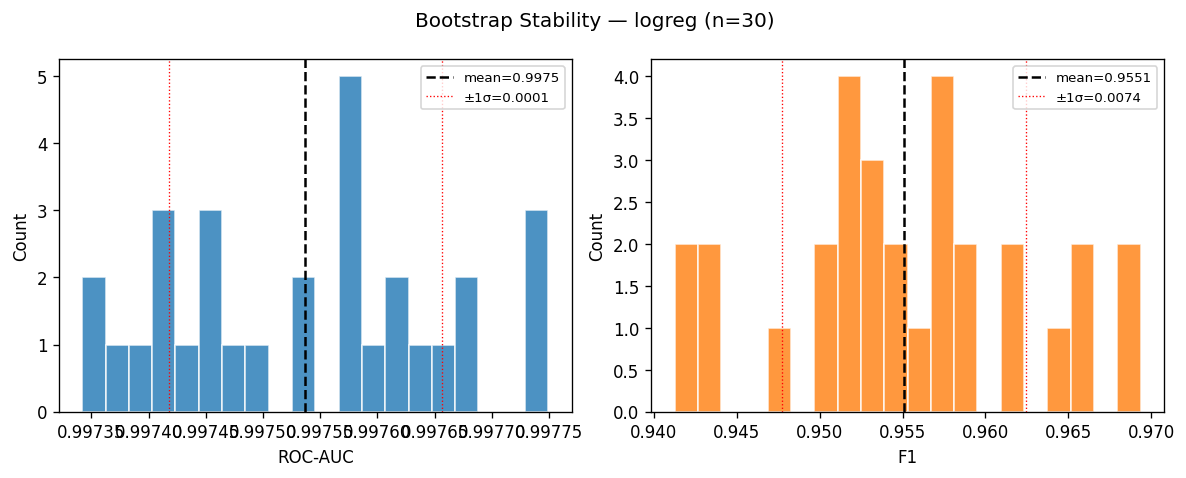
\includegraphics[width=0.85\textwidth]{figures/stability_bootstrap_logreg.png}
\caption{Bootstrap stability (30 iterations). ROC-AUC (left) and F1 (right) distributions are tightly concentrated.}
\label{fig:stability_bootstrap}
\end{figure}

Figure~\ref{fig:stability_noise} shows that, under perturbations with noise at $\sigma = 0.5$ (50\% of feature standard deviation), ROC-AUC remains above 0.98. F1 degrades a little more, but discriminative ability is preserved.

\begin{figure}[H]
\centering
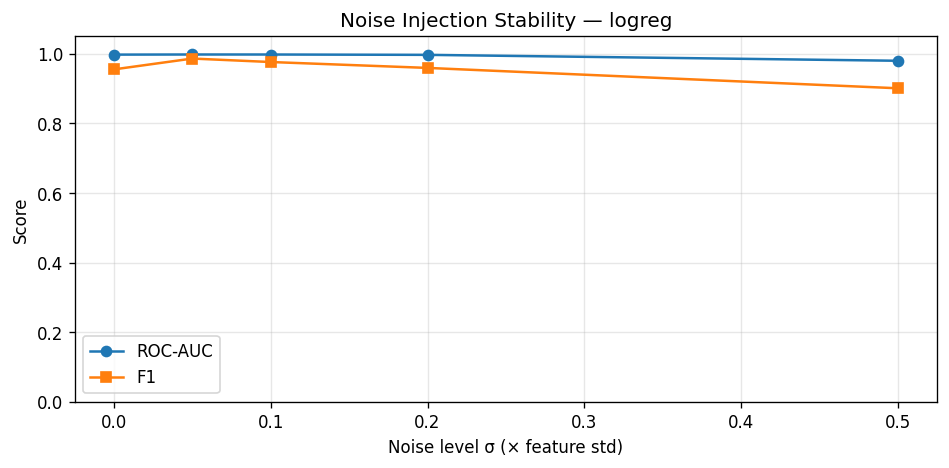
\includegraphics[width=0.55\textwidth]{figures/stability_noise_logreg.png}
\caption{Noise injection stability. ROC-AUC (blue) is robust to moderate noise; F1 (orange) is more sensitive due to threshold effects.}
\label{fig:stability_noise}
\end{figure}

Under different winsorization levels, the 1\%--99\% setting achieves the best F1 (0.980). This is displayed in Figure~\ref{fig:stability_preproc}. Even aggressive clipping at 10\%--90\% only drops AUC from 0.998 to 0.993. These results justify our choice of clipping.

\begin{figure}[H]
\centering
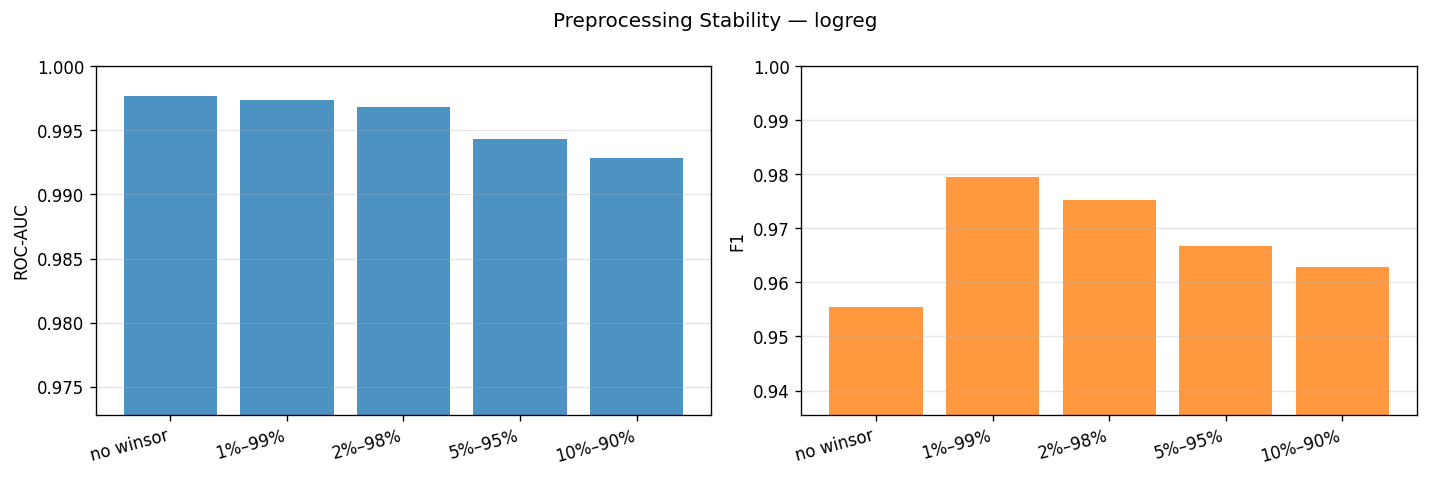
\includegraphics[width=0.85\textwidth]{figures/stability_preprocessing_logreg.png}
\caption{Preprocessing stability: ROC-AUC (left) and F1 (right) across winsorization levels.}
\label{fig:stability_preproc}
\end{figure}


\subsubsection{Predictions on Unlabeled Images}

Our ultimate goal is to have the logistic regression model be able to predict the presence of clouds on all 164 images in the dataset. Figure~\ref{fig:cloud_hist} shows the distribution of predicted cloud fractions, which is bimodal with peaks at low ($<$10\%) and high ($>$90\%) coverage. The three labeled images (red bars) fall in the 30--50\% range, missing the extreme values of images that have either next to no clouds or are mostly made up of clouds. The model has never trained on near-clear or fully-overcast scenes, so its predictions on those images are extrapolated. Providing more expert-labeled images that are in these extremes will help with the model in the long run.

\begin{figure}[H]
\centering
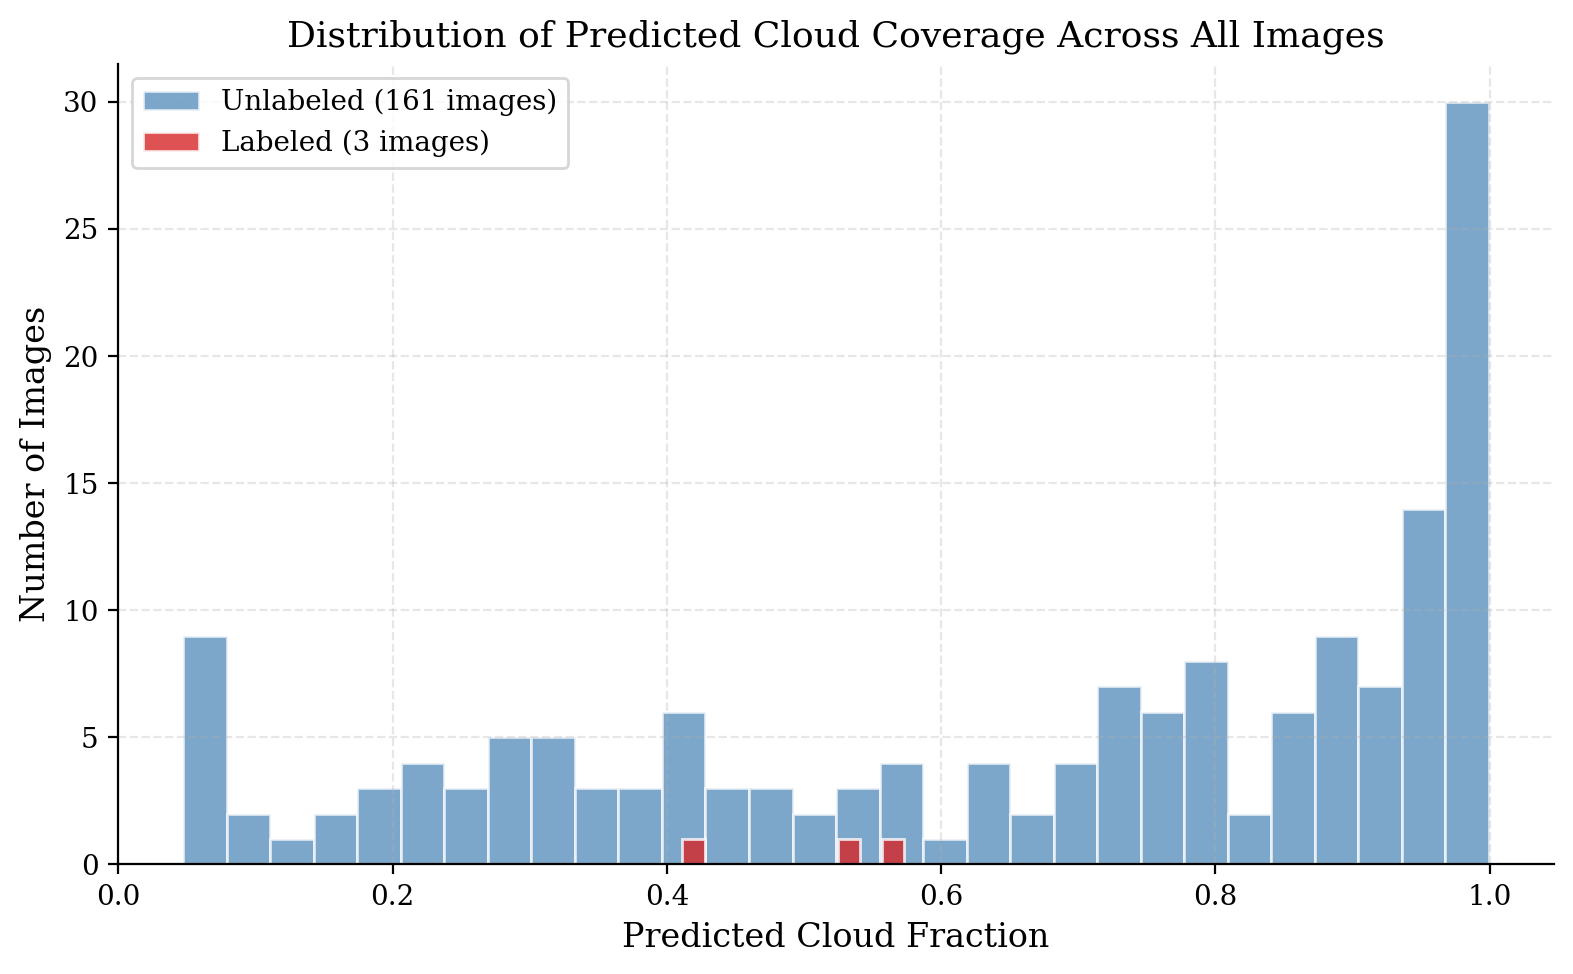
\includegraphics[width=0.65\textwidth]{figures/cloud_fraction_histogram.png}
\caption{Distribution of predicted cloud fraction across all 164 images. Red bars mark the 3 labeled images.}
\label{fig:cloud_hist}
\end{figure}

Figure~\ref{fig:unlabeled_gallery} shows predicted cloud masks for a sample of unlabeled images. The predictions are spatially coherent with smooth cloud boundaries.

\begin{figure}[H]
\centering
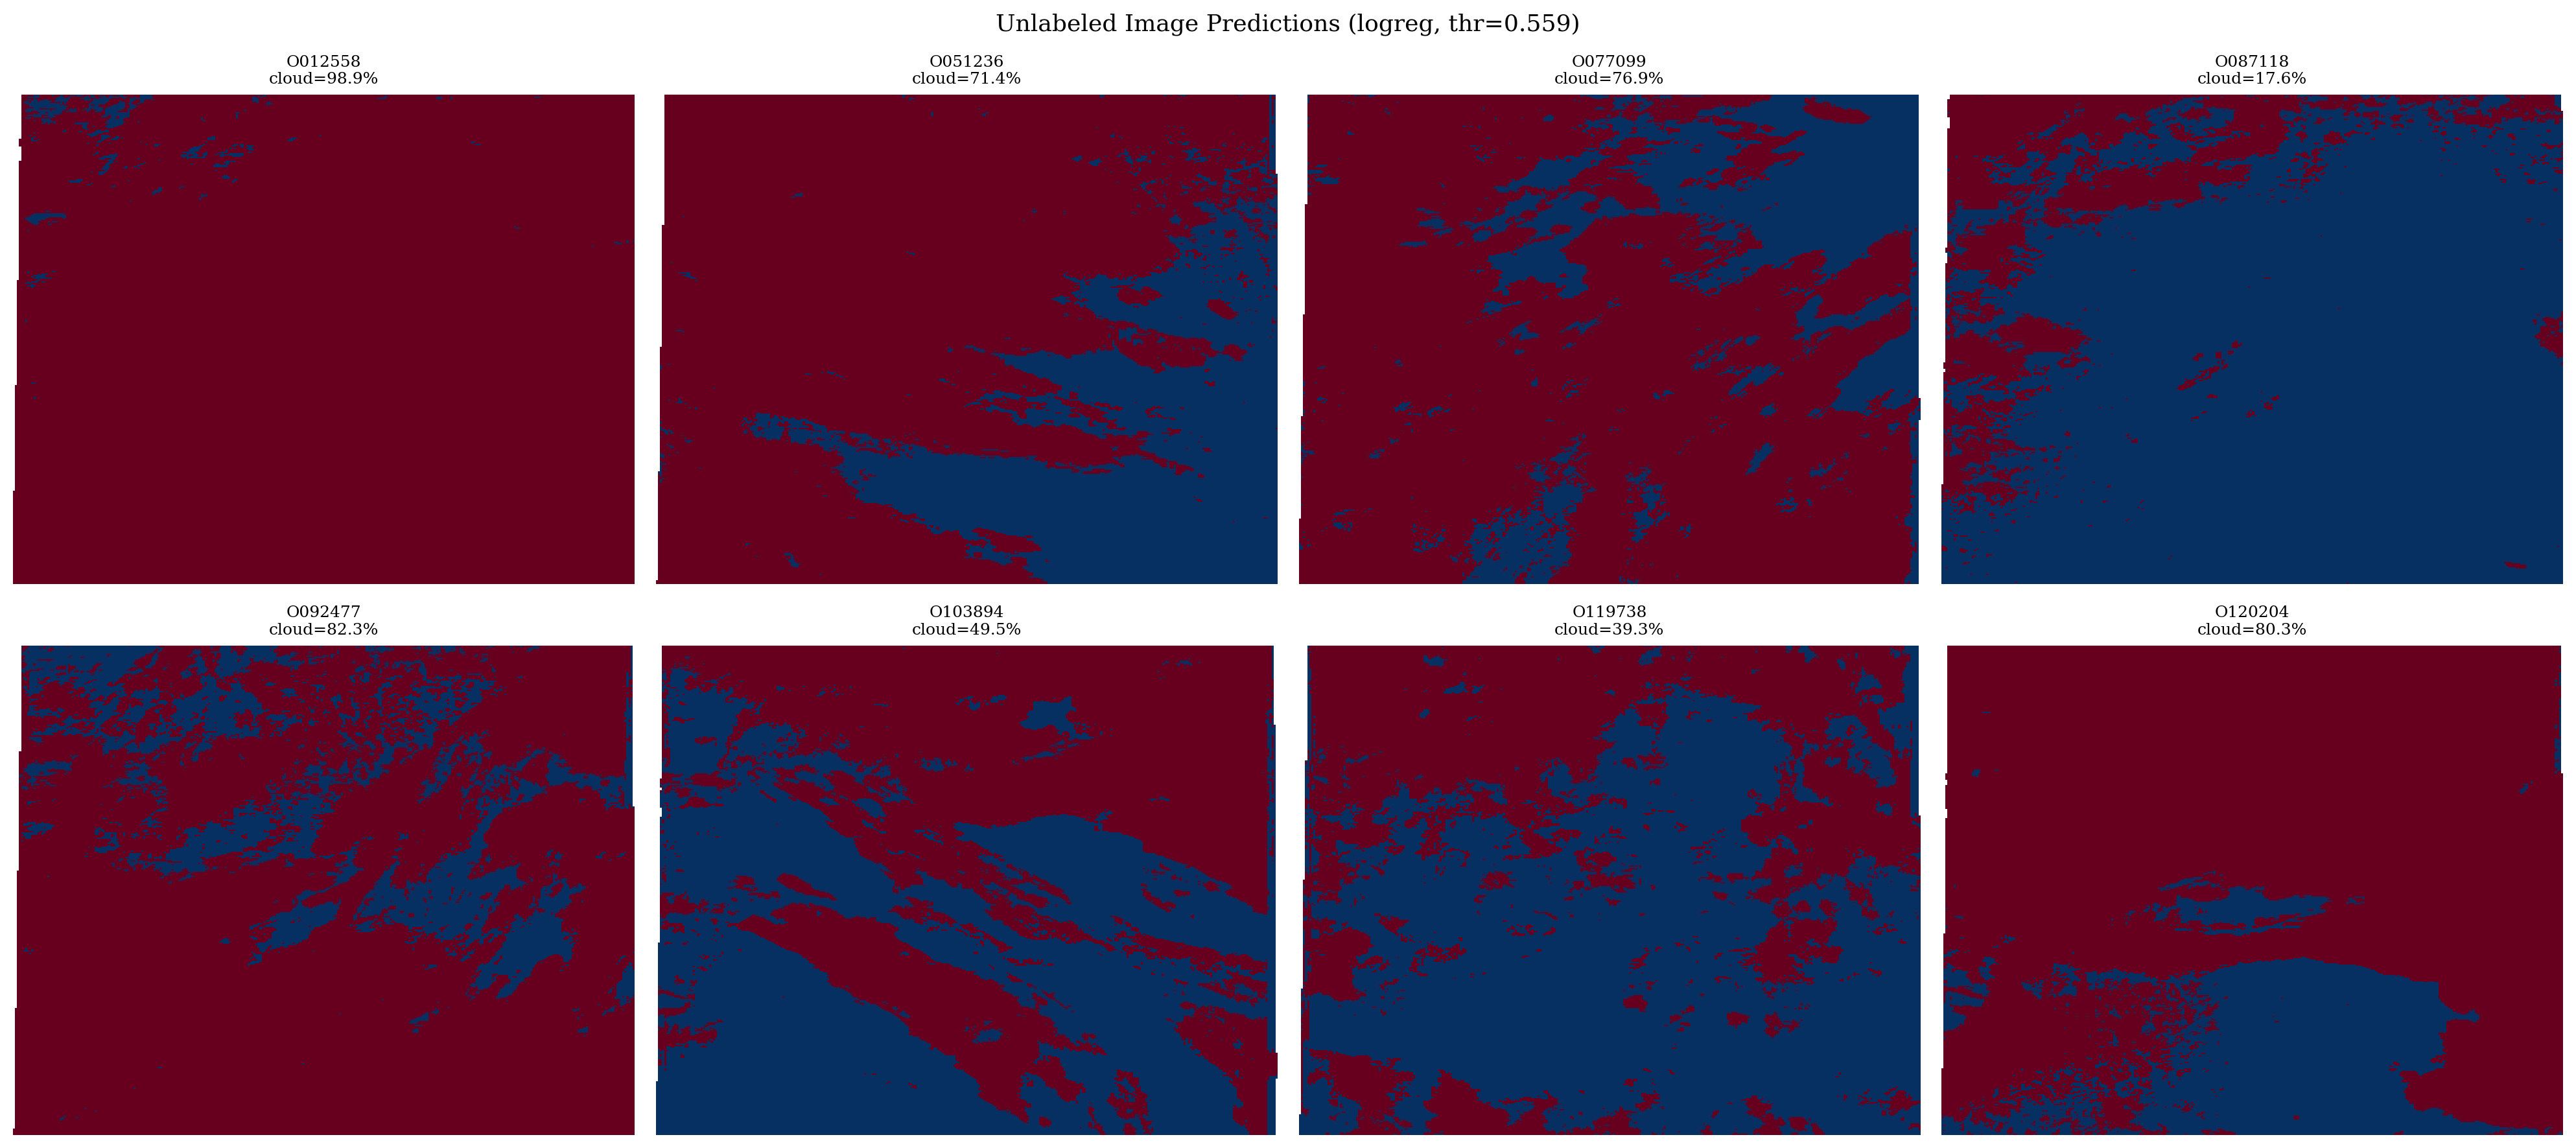
\includegraphics[width=0.75\textwidth]{figures/unlabeled_predictions_logreg.png}
\caption{Predicted cloud masks for selected unlabeled images (logistic regression). Red = cloud, blue = non-cloud.}
\label{fig:unlabeled_gallery}
\end{figure}

\subsubsection{Spatial Error Analysis}

Figure~\ref{fig:error_map} shows the spatial error map for GBM on Split~1. Colored by instances of true positives, true negatives, false positives, and false negatives. The darker gray regions of the plot are pixels that are not expert-labeled, and therefore we are unable to to label them as TP, TN, FP, or FN.

\begin{figure}[H]
\centering
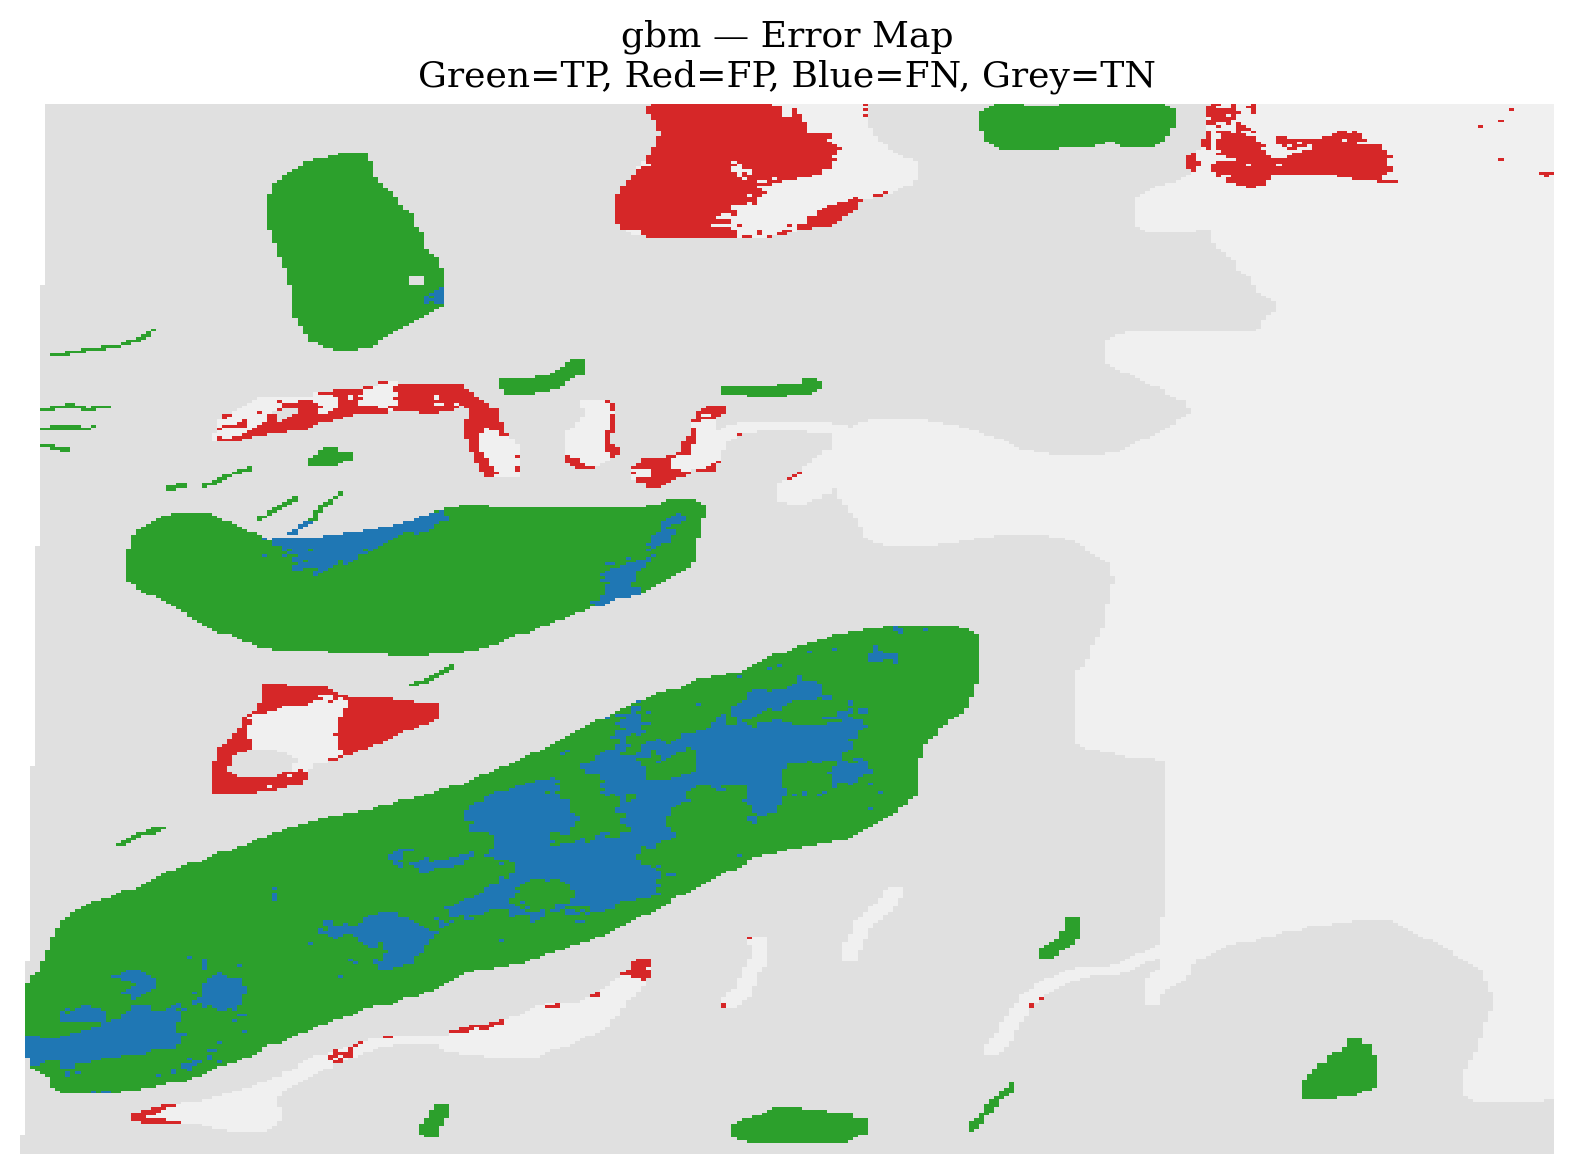
\includegraphics[width=0.55\textwidth]{figures/fold_1/spatial_error_map_gbm.png}
\caption{Spatial error map for GBM on the Split~1 test image (O012791). Green = TP, light-gray = TN, red = FP, blue = FN. Errors concentrate at cloud boundaries.}
\label{fig:error_map}
\end{figure}

We can identify several places where false negatives (blue) occur on the boundaries of true positive (green). These are places where the separation between a cloud at it's boundaries and the ground beneath it is harder to ascertain. Whereas false positives (red) occur on areas of bright ice that mimics cloud reflectance. Let's compare the spatial errors in Figure~\ref{fig:error_map} with the probability heatmaps for GBM and logistic regression. 

Figure~\ref{fig:prob_heatmap} shows predicted cloud probabilities for Logistic Regression and Gradient Boosting models on Split~1. i.e. the probability that a pixel is either a cloud or not decided by the model. The GBM produces sharper transitions while the transitions from logistic regression's predictions are smoother. The end result of the GBM model is a more confident (sometimes more confidently wrong) model of discerning the presence of cloud in a pixel.

\begin{figure}[H]
\centering
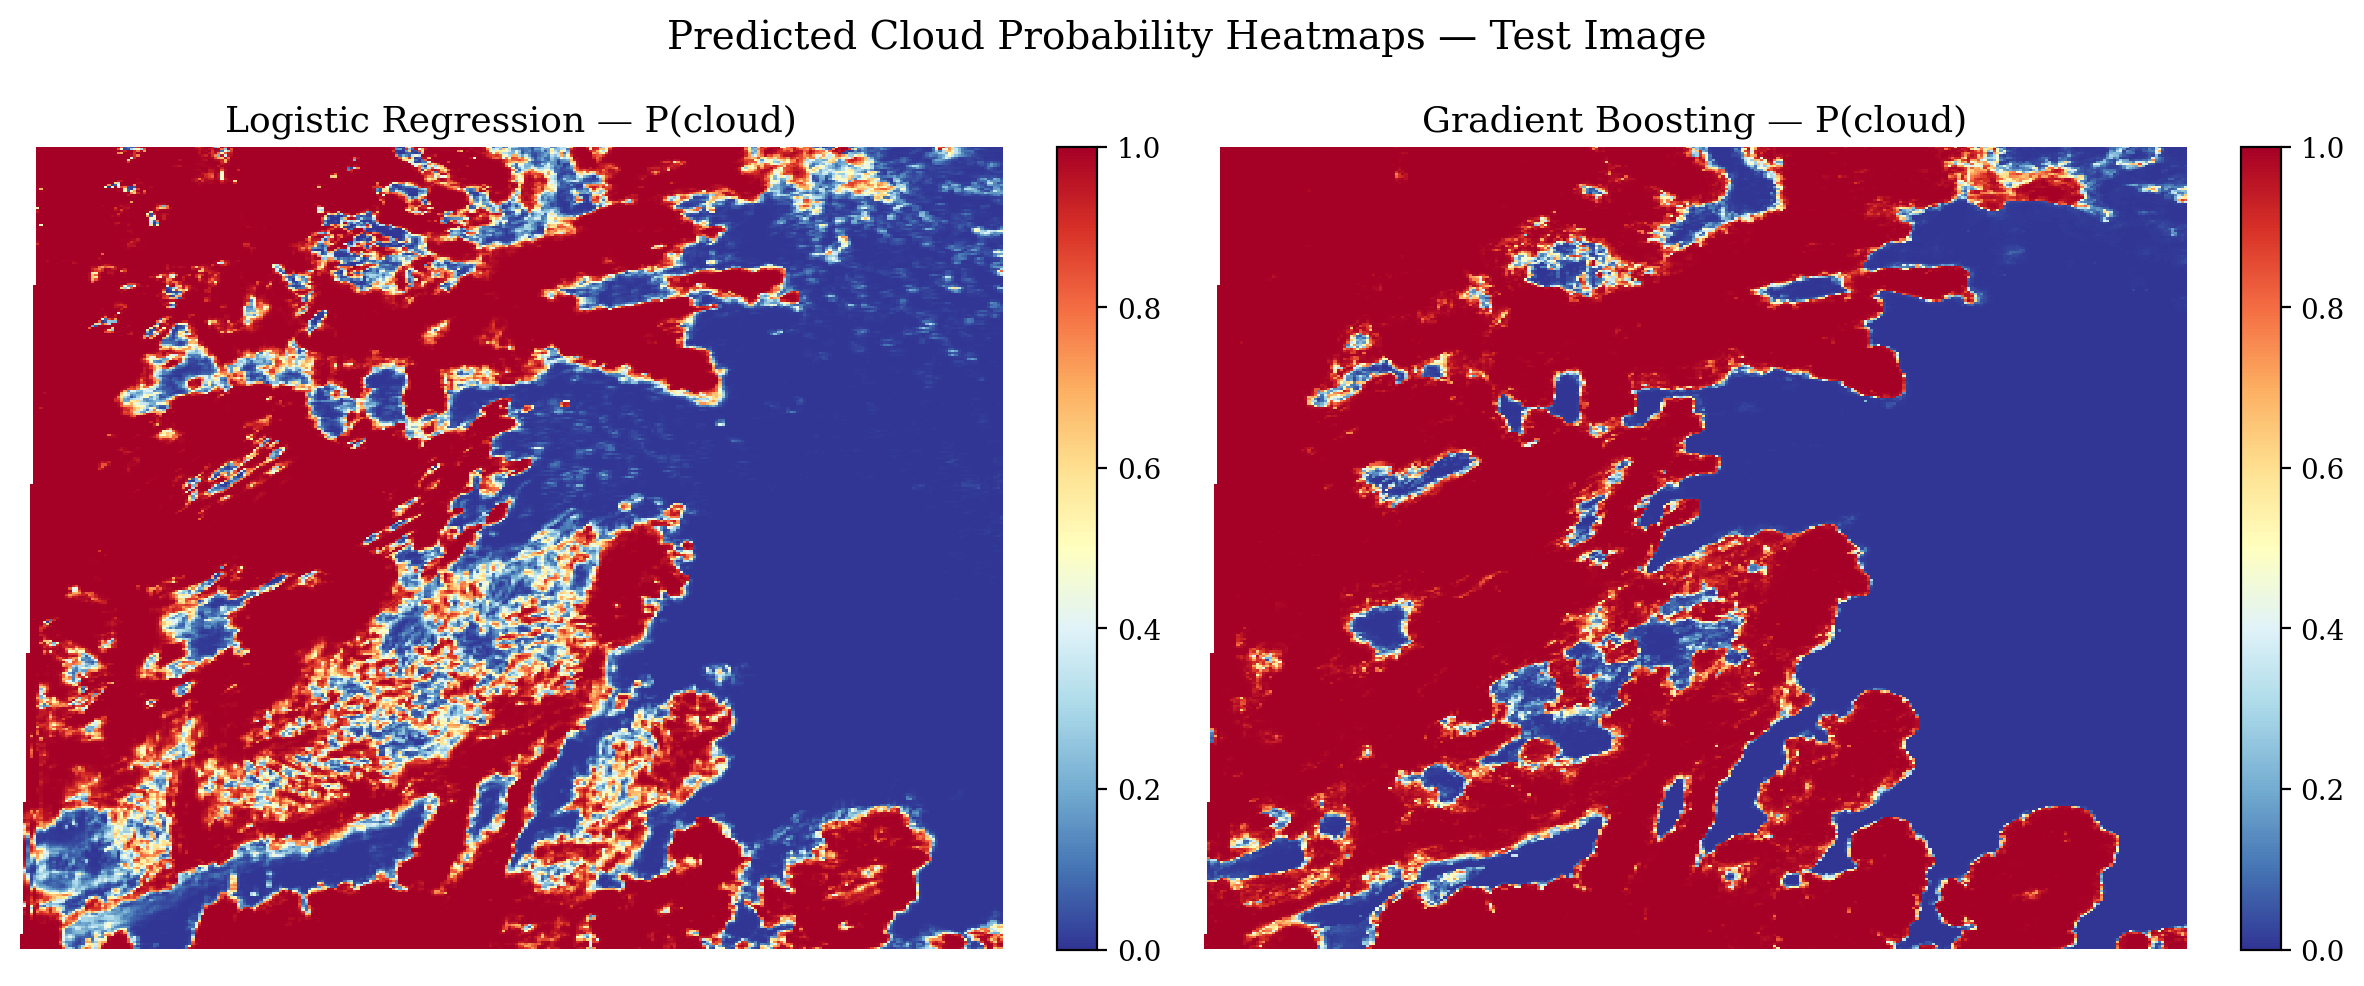
\includegraphics[width=\textwidth]{figures/fold_1/spatial_probability_heatmaps.png}
\caption{Predicted cloud probability heatmaps for the Fold~1 test image. Warmer colors indicate higher cloud probability.}
\label{fig:prob_heatmap}
\end{figure}

Given the behavior in the plots above, we would suggest that, instead of using a hard, if adaptive, threshold on the probability to assign cloud or no cloud, we assign pixels with certain probabilities \textbf{no label}. This would mirror the expert-labeled images presented in Figure~\ref{fig:expert_labels}, as even the best human judgment leaves many pixels unlabeled.







\section{Conclusion}
\label{sec:conclusion}

Our goal is to better understand the mechanisms behind the data collected by MISR technology and how they can be leveraged to detect clouds over the Arctic region. We began by conducting an exploratory data analysis, where we found that while both the radiation measurements and the expert-derived features can be used to detect clouds, there are differences between images, which pose a challenge given the limited amount of labeled data we have. For this reason, we outlined a data splitting methodology that allowed us to analyze the choice of training/testing images when we conducted our predictive modeling.

Next, we conducted feature engineering and feature extraction. We developed many ideas for transforming the features and found that the most effective ones used a combination of expert-derived features and spatial structure by looking at a patch of data. Additionally, we built an autoencoder using all images to perform feature extraction, which supplemented the features that we engineered.

We then built four predictive models for cloud detection: a logistic regression model, random forest model, gradient boosting model, and $k$-Nearest Neighbors classifier. We found that the logistic regression model had the best combination of performance and consistency across splits, but that the GBM can also provide additional predictive power at the cost of consistency. Additionally, while the features that we engineered complemented the features extracted by the autoencoder, many of them ended up being redundant and could've been discarded at the cost of little predictive power.

Finally, we concluded our work with a discussion on the limitations of our models. We found that many of the misclassifications occurred at cloud boundaries and had predicted probabilities that were in the middle range, representing high uncertainty. It is for this reason that we proposed flagging pixels with probabilities in this range as uncertain, rather than cloud/no-cloud, as even experts were not able to discern between clouds for some regions.



\newpage

\section{Bibliography}

\begin{thebibliography}{9}

\bibitem{Shi}
Shi, T., Yu, B., Clothiaux, E. E., \& Braverman, A. J. (2008). Daytime Arctic Cloud Detection Based on Multi-Angle Satellite Data With Case Studies. \textit{Journal of the American Statistical Association, 103}(482), 584–593. https://doi.org/10.1198/016214507000001283

\bibitem{Gonzalez}
Gonzalez, R. C., \& Woods, R. E. (2019). \textit{Digital Image Processing}. Pearson

\bibitem{Yu}
Yu, B., \& Barter, R. (2024). \textit{Veridical Data Science: The Practice of Responsible Data Analysis and Decision Making}. MIT Press

\end{thebibliography}

\appendix
\section{Academic honesty}

\subsection{Statement}

To Professor Bin Yu, we pledge that this report represents our own original work and analysis. All sources, including datasets, code libraries, and reference materials, are properly cited. We have not shared our code or written work with other groups, nor have we copied from any external source. We believe academic honesty is essential because the integrity of scientific research depends on transparent and truthful reporting of methods and results. Fabricated or misrepresented findings undermine the trust that the scientific community and the public place in research outcomes.

\subsection{LLM Usage}

\subsubsection*{Coding}
LLM tools (GitHub Copilot, Claude) were used to assist with boilerplate code for data loading, visualization functions, and SLURM job scripts. All code was reviewed, edited, and tested by the team members to ensure correctness and alignment with our analysis goals.

\subsubsection*{Writing}
LLM assistance was used for grammar correction, to help structure section outlines, and to sanity check some formulas. The substantive content, analysis, interpretations, and scientific arguments in this report are our own.

\end{document}
